\documentclass[12pt]{report}
\pagestyle{headings}

% Note that the line below could be modified to suit a
% particular system since the "geometry" package behaves
% differently in Unix, Windows and Mac, especially for the
% top margins.
% Adjust the parameter "top" (measuring the height of the
% space allocated to a header) and "headsep" (measuring
% the distance from the bottom of the header to the
% first line of text.
\usepackage[top=1.3in,left=1.5in,bottom=1in,right=1in,headsep=0.5in]{geometry}

\usepackage{setspace}
\onehalfspacing
%\doublespacing

% Headers and footers for thesis
\usepackage{fancyhdr}

\markboth{}{}
\newcommand\startchapter[1]{\chapter{#1}\thispagestyle{myheadings}}
\newcommand\startappendix[1]{\chapter{#1}\thispagestyle{myheadings}}
\newcommand\startfirstchapter[1]{\chapter{#1}}

% Manual addition of section to Table of Contents
\newcommand\TOCadd[1]{\newpage\phantomsection\addcontentsline{toc}{chapter}{#1}}

% Float Customization
\renewcommand{\floatpagefraction}{0.01}

% Customization of Tables of Contents and List of Figures/Tables
\usepackage{tocloft}
\renewcommand\cfttabpresnum{Table\ }
\renewcommand\cfttabnumwidth{0.75in}
\renewcommand\cftfigpresnum{Figure\ }
\renewcommand\cftfignumwidth{0.80in}
\newcommand{\HRule}{\rule{\linewidth}{0.5mm}}


% Long Table and decimal aligned columns
\usepackage{dcolumn}
\usepackage{longtable}

% Mathematics support
\usepackage{amsmath}
\usepackage{amsthm}
\usepackage{amssymb}


% Text Control
\usepackage{xspace}
\usepackage{textcase}

% Graphics
\usepackage{wasysym}
\usepackage{graphics}
\usepackage{graphicx}   % A package to allow insertion of
                        % external image files


\newcommand*{\pt}{$p_\text{T}$\xspace}
\newcommand*{\etmiss}{$E_\text{T}^\text{miss}$\xspace}
\newcommand*{\etmissvec}{$\vec{E}_\text{T}^\text{miss}$\xspace}
\newcommand*{\chichi}{$\chi\bar{\chi}$\xspace}
\newcommand*{\monoZ}{mono-$Z$\xspace}
\newcommand*{\MonoZ}{Mono-$Z$\xspace}
\newcommand*{\pp}{$pp$\xspace}
\newcommand*{\Z}{$Z$\xspace}
\newcommand*{\monoZll}{mono-$Z(\ell\ell)$\xspace}
\newcommand*{\MonoZll}{Mono-$Z(\ell\ell)$\xspace}
\newcommand*{\monoX}{mono-$X$\xspace}
\newcommand*{\ee}{$ee$\xspace}
\newcommand*{\epem}{$e^+ e^-$\xspace}
\newcommand*{\mm}{$\mu\mu$\xspace}
\newcommand*{\mpmm}{$\mu^+ \mu^-$\xspace}
\newcommand*{\Zlletmiss}{$Z(\ell\ell)+E_T^\text{miss}$\xspace}
\newcommand*{\Zetmiss}{$Z+E_T^\text{miss}$\xspace}
\newcommand*{\mchi}{$m_\chi$\xspace}
\newcommand*{\mmed}{$m_\text{med}$\xspace}
\newcommand*{\etmissX}{$E_T^\text{miss}+X$\xspace}
\newcommand*{\qq}{$q\bar{q}$\xspace}
\newcommand*{\Wmed}{$\Gamma_\text{med}$\xspace}
\newcommand*{\gq}{$g_q$\xspace}
\newcommand*{\gchi}{$g_\chi$\xspace}
\newcommand*{\Zjets}{$Z$+jets\xspace}
\newcommand*{\gjets}{$\gamma$+jets\xspace}
\newcommand*{\ifb}{fb$^{-1}$\xspace}
\newcommand*{\madgraph}{\textsc{MadGraph}\xspace}
\newcommand*{\pythia}{\textsc{Pythia}\xspace}
\newcommand*{\etmisspar}{$E_{T,||}^\text{miss}$\xspace}
\newcommand*{\etmissht}{$E_T^\text{miss}/H_T$\xspace}

\usepackage[T1]{fontenc}
\usepackage{graphicx}
\usepackage{subcaption}
\usepackage{color}
\usepackage{xcolor}
%\usepackage{biblatex}
%\addbibresource{bibliography.bib}

\begin{document}

% Front Matter
\input frontmatter/fm

\newpage

	\startfirstchapter{Introduction}
\label{chapter:introduction}

The Standard Model (SM) of particle physics is the most complete theory that exists to describe elementary particles and their interactions. However there are known weaknesses in the SM, one of which is the failure to include a description of dark matter (DM). There is strong evidence from astronomical observations that there is a large excess of matter in the universe that appears to have only gravitational interactions with SM particles. Some examples for the evidence of dark matter include measurements of rotation velocities of spiral galaxies, gravitational lensing effects, and anisotropies in the cosmic microwave background. The standard model of cosmology predicts that dark matter accounts for approximately 27\% of the total mass energy of the universe. Although there are many theories to describe possible dark matter candidates, the one of interest here is the WIMP (weakly interacting massive particle). The WIMP is a Dirac fermion, often denoted $\chi$, and is predicted to interact gravitationally and through other force(s), potentially beyond the SM. It is predicted to have a mass between 10 GeV and a few TeV, and have a self-annihilation cross section similar to that of SM weak interactions.

There are three categories of experiments that have potential to observe dark matter: direct detection, indirect detection, and collider production. Figure \ref{fig:detection} shows a schematic that illustrates their complementarity to one another. Direct detection (DD) experiments attempt to observe recoils in SM particles from scattering with dark matter. Indirect detection (ID) experiments measure decay products from DM annihilation. Collider experiments look for dark matter that is is produced from the annihilation of SM particles. This work focuses on the production of dark matter at the Large Hadron Collider (LHC) using data collected from proton-proton (\pp) collisions inside the ATLAS detector.

\begin{figure}[htb]
\centering
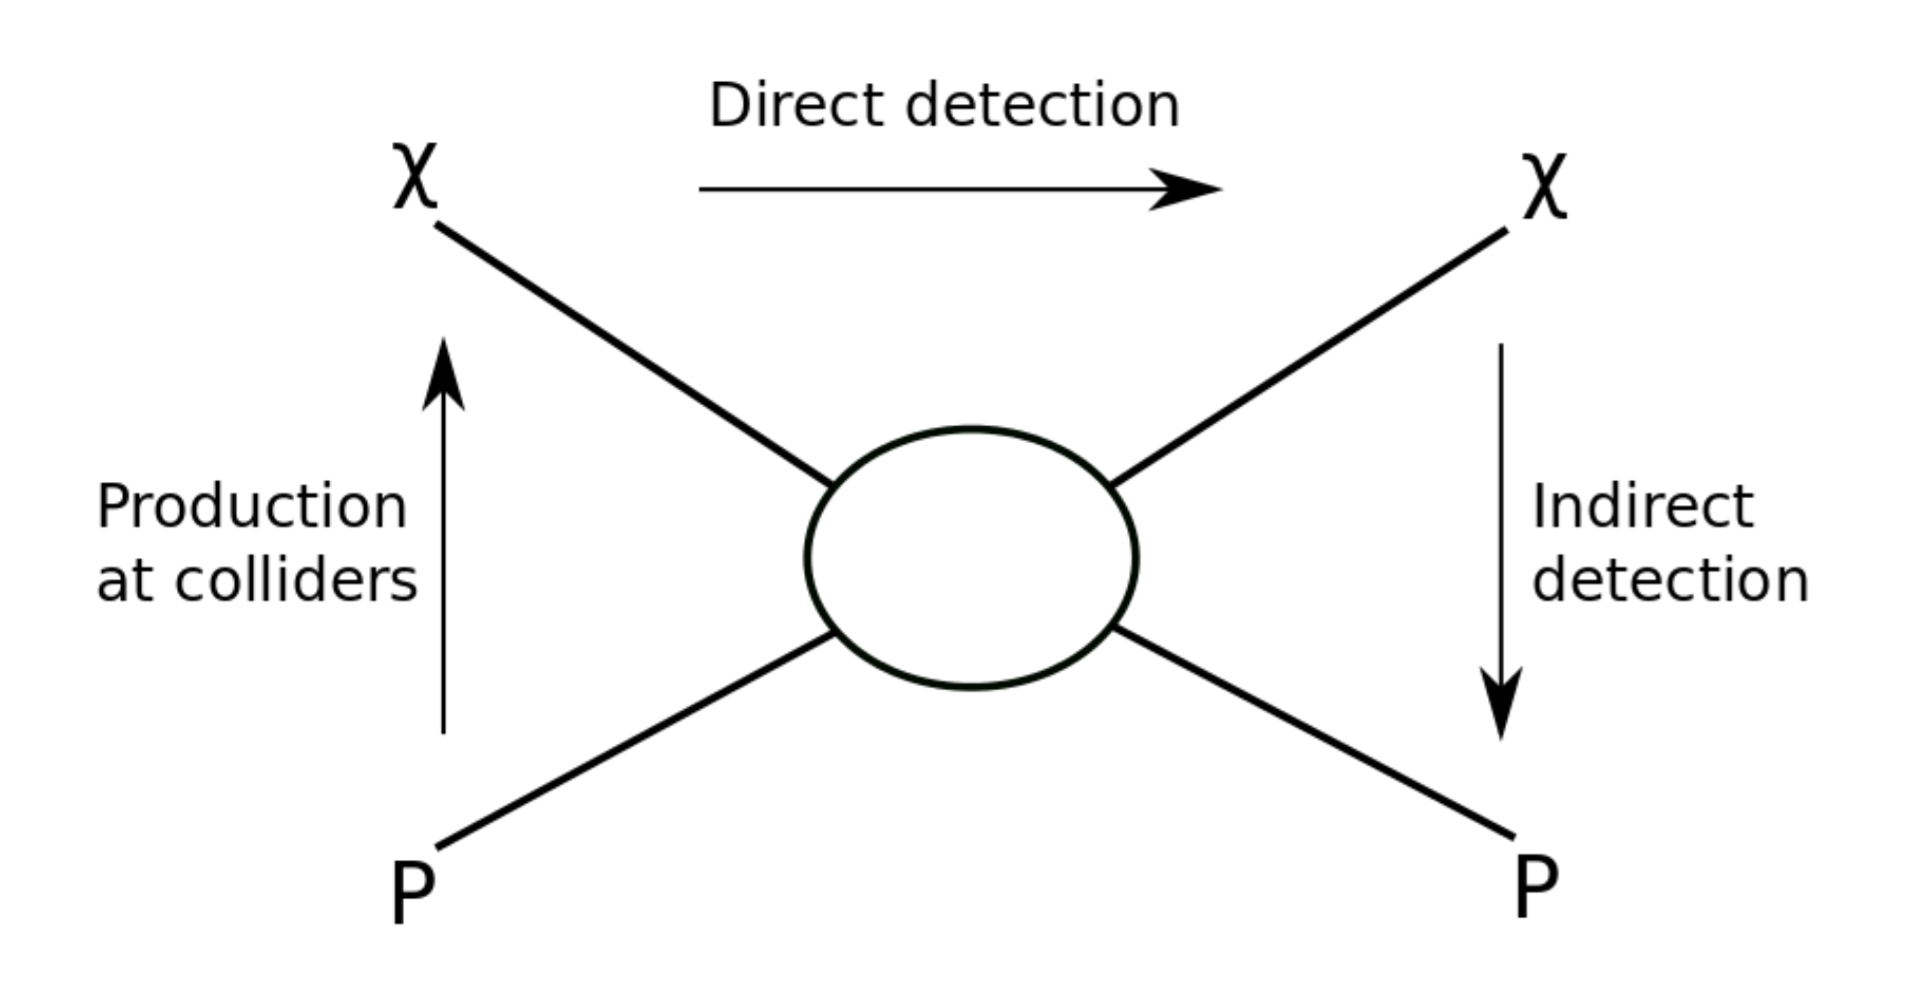
\includegraphics[width=0.6\textwidth]{Figures/detection.png}
% https://arxiv.org/pdf/1509.08767.pdf
\caption{Schematic of potential dark matter interactions and their experimental categories. {\color{red}TODO: Citation!}}
\label{fig:detection}
\end{figure}

If it is possible to produce dark matter in collisions of SM particles, then an additional complication is how the presence of dark matter can be determined in a very dense environment of high energy particles. Collider experiments use a quantity known as missing transverse momentum, or missing transverse energy, commonly denoted \etmiss, to quantify the amount of invisible decay products in collisions. The plane perpendicular to the beam axis, also known as the transverse plane, is of particular importance in collider experiments. Before colliding, the protons in the beam only move along the beam axis, so the net momentum in the transverse plane is zero. From conservation of momentum, the net transverse momentum after the collision therefore must also be zero. If the transverse momenta of all visible particles produced in the collision are added together vectorially, they should add to zero. But, if invisible particles are present, such as neutrinos or dark matter, then the sum will instead add to a non-zero transverse momentum vector. We therefore infer that there are non-interacting particles produced, and they have a net \etmiss vector that is the negative of the vectorial sum of the transverse momenta of the visible particles. Hence a dark matter signal would manifest as an excess of collision events with a significant amount of \etmiss compared to the SM prediction.

In order to pick out events with a large amount of \etmiss, another (visible) particle must be used as a `tag.' If the amount of missing energy in an event is large, the tag particle will experience a significant amount of recoil against the \etmiss vector. This gives a mean of identifying potentially interesting events. In this work the \Z boson is used as a tag, which is identified in events from a pair of same sign, opposite charge leptons (\epem or \mpmm). This analysis attempts to find dark matter with \Zlletmiss events, and is therefore commonly referred to as the \monoZll search. Other mono-$X$ searches use different SM particles as tags, such as a jet, photon, $H$, or $W$.

The ATLAS experiment has been in a period of intense data-taking since the start of Run 2 in 2015, with \pp collisions at a centre-of-mass energy of 13 TeV. As data continues to be collected until the end of 2018, the discovery potential for dark matter at the LHC has never been higher. This document summarizes the work done on the \monoZll analysis so far as well as the prospects for the full Run 2 dataset. Chapter \ref{chapter:theory} includes a summary of the dark matter models considered in the analysis, as well as a brief description of the LHC and the ATLAS detector. Chapter \ref{chapter:prevWork} covers the details of the search with a focus on the work done for the results obtained using the 2015 and 2015+2016 datasets. Chapter \ref{chapter:fullRun2} describes the plan to analyze the complete Run 2 dataset over the full period from 2015-2018.



	\startchapter{Dark Matter Searches with the ATLAS Detector}
\label{chapter:theory}

% --------------------------------------------------------------------------------------
\section{Dark Matter Theory}

Effective field theories (EFTs) \cite{Boveia:2016mrp} \cite{Carpenter:2012rg} were the primary models studied in \etmissX dark matter searches in Run 1, when the centre-of-mass energy was 8 TeV. In short, these theories assume that a dark matter pair is produced by means of a contact interaction with a quark and antiquark, as illustrated in Figure \ref{fig:efts}. These types of models offer a straightforward means to compare collider results to direct or indirect detection experiments. However, EFTs are only valid when the mass of the mediating particle between the \chichi and \qq is much heavier than the momentum transfer of the process. Now that the centre-of-mass energy has increased to 13 TeV in Run 2, these EFTs are no longer valid. Thus, a new baseline model is used in Run 2 with the mediator particle explicitly included.

\begin{figure}[htb]
    \centering
    \selectcolormodel{gray}
    \begin{subfigure}[b]{0.35\textwidth}
        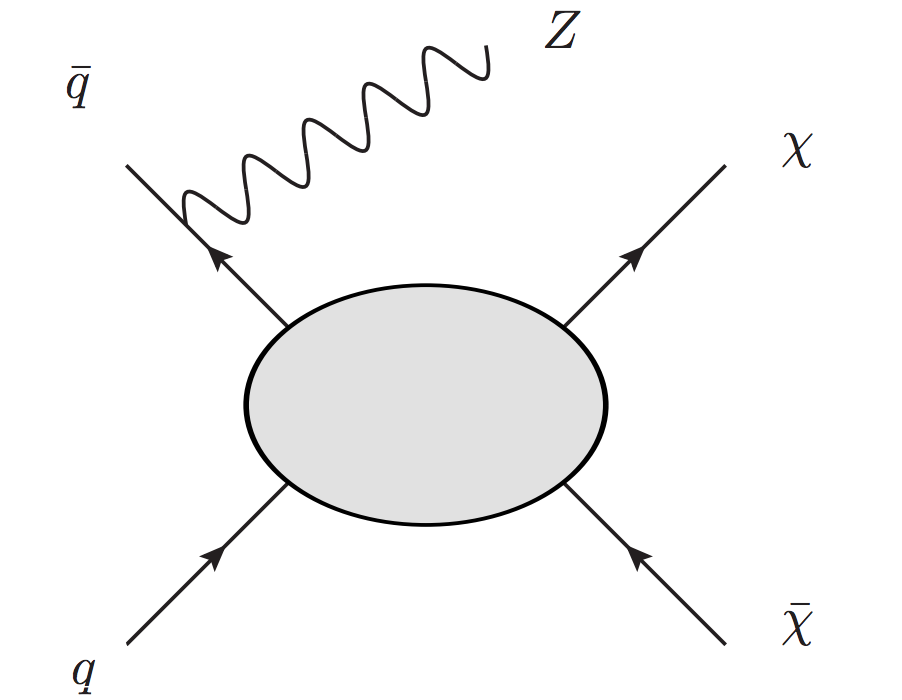
\includegraphics[width=\textwidth]{Figures/eft1.png}
        \label{fig:eft1}
    \end{subfigure}
    ~ %add desired spacing between images, e. g. ~, \quad, \qquad, \hfill etc. 
      %(or a blank line to force the subfigure onto a new line)
    \begin{subfigure}[b]{0.35\textwidth}
        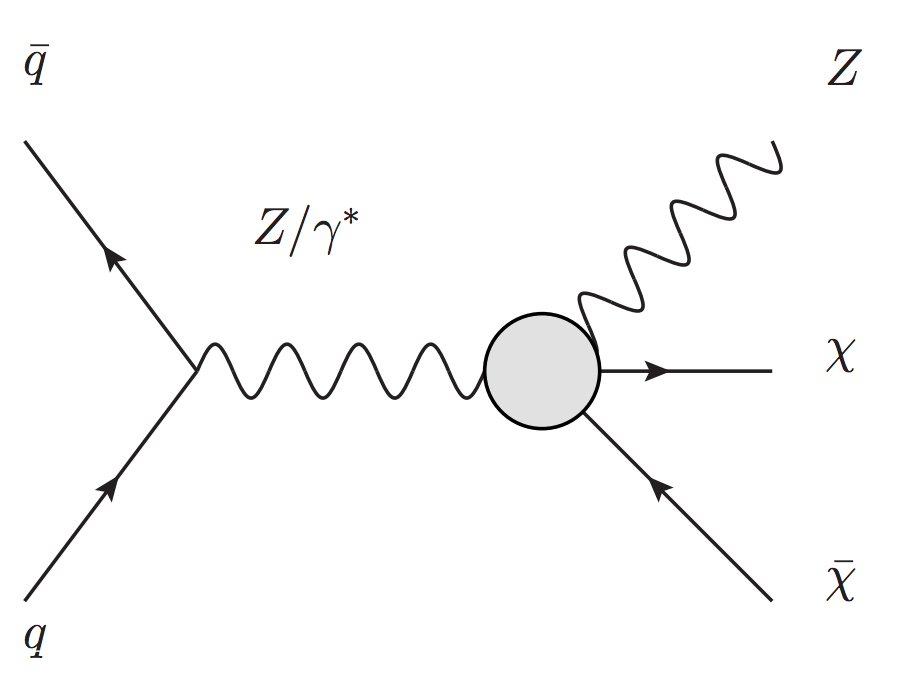
\includegraphics[width=\textwidth]{Figures/eft2.png}
        \label{fig:eft2}
    \end{subfigure}
    \caption{Representative EFT diagrams for the \monoZ signature \cite{Carpenter:2012rg}.}
\label{fig:efts}
\end{figure}

Leading order simplified models are the first set of benchmark models used for \etmissX searches in Run 2, as recommended by the LHC DM Working Group \cite{Boveia:2016mrp}. An example $s$-channel diagram for the \Zetmiss signal is shown in Figure \ref{fig:simp}. These models are considered `simplified' because they introduce the minimum number of parameters needed to include a mediator between SM and dark matter particles (compared to more complicated models such as supersymmetry). 

\begin{figure}[htb]
\centering
\selectcolormodel{gray}
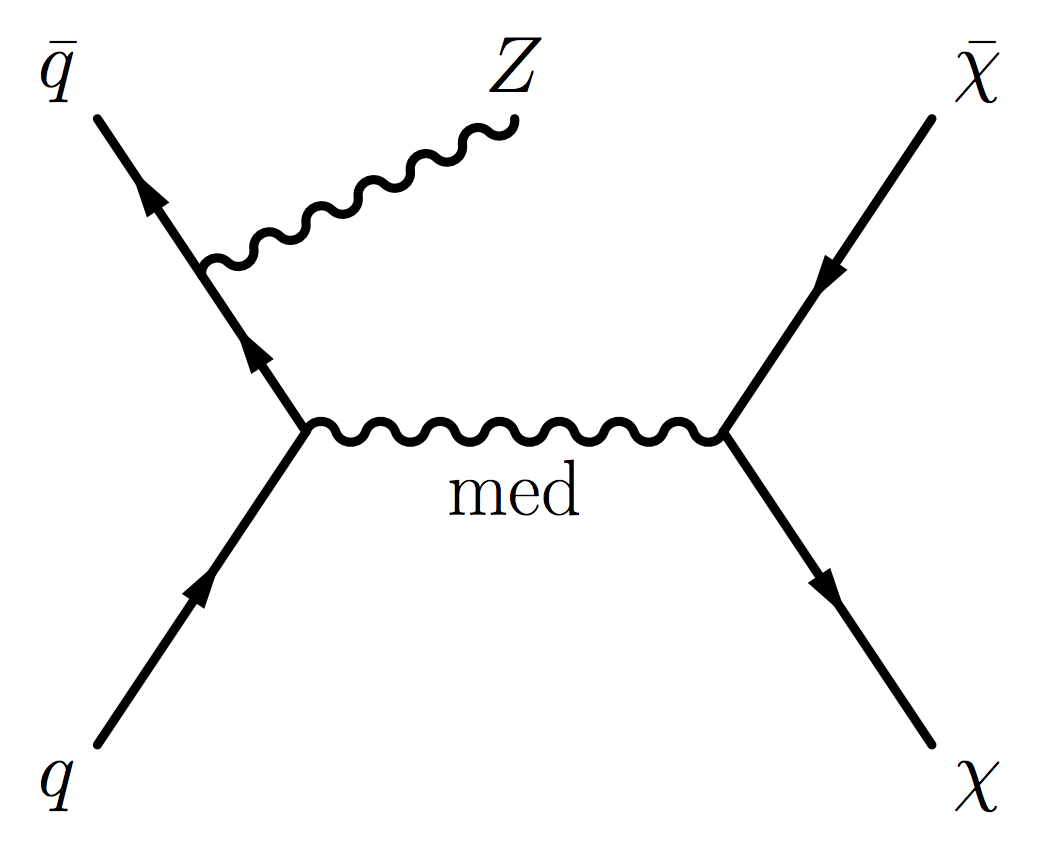
\includegraphics[width=0.3\textwidth]{Figures/simp.png}
\caption{Simplified model $s$-channel diagram for the \monoZ signature \cite{Aaboud:2017bja}.}
\label{fig:simp}
\end{figure}

Simplified models introduce five new parameters: the mass of the WIMP, \mchi, the mass of the mediating particle, \mmed, the couplings of the mediator to the SM (to dark matter), \gq (\gchi), and the width of the mediator \Wmed. The mediator particle can be spin-0 (scalar or pseudo-scalar) or spin-1 (vector or axial-vector). 

%The interaction Lagrangians for models with vector and axial-vector mediator couplings are given in Equations \ref{eqn:Lvector}, and \ref{eqn:Laxial}:

%\begin{equation}
%\mathcal{L}_\text{vector} = g_q \sum_q \eta_\mu \bar{q} \gamma^\mu q + g_\chi \eta_\mu \bar{\chi} \gamma^\mu \chi
%\label{eqn:Lvector}
%\end{equation}

%\begin{equation}
%\mathcal{L}_\text{axial-vector} = g_q \sum_q \eta_\mu \bar{q} \gamma^\mu \gamma^5 q + g_\chi \eta_\mu \bar{\chi} \gamma^\mu \gamma^5\chi
%\label{eqn:Laxial}
%\end{equation}

Following the recommendations in Ref.\ \cite{Boveia:2016mrp}, for spin-0 models the couplings are set to \gq~=~\gchi~=~1.0. The Yukawa couplings are also included between the quarks and the mediator. For spin-1 models the couplings are fixed to $g_q = 0.25$ and $g_\chi = 1.0$. In addition, assuming that the mediator has no additional decay modes, \Wmed is set to the minimal width \cite{Abercrombie:2015wmb}, which is fixed by \gq, \gchi, \mchi, and \mmed. The couplings were chosen so that \Wmed/\mmed < $\sim$0.05, and to correspond approximately to an estimate of the lower sensitivity of the Run 2 mono-jet analysis.

%Similarly, the interaction Lagrangians for models with scalar and pseudo-scalar mediator couplings are given by Equations \ref{eqn:Lscalar} and \ref{eqn:Lpseudo}:

%\begin{equation}
%\mathcal{L}_\text{scalar} = g_\chi \eta \bar{\chi} \chi + \frac{\eta}{\sqrt{2}} g_q \sum_i \left( y_i^u \bar{u}_i u_i + y_i^d \bar{d}_i d_i + y_i^\ell \bar{\ell}_i \ell_i \right)
%\label{eqn:Lscalar}
%\end{equation}

%\begin{equation}
%\mathcal{L}_\text{pseudo-scalar} = i g_\chi \eta \bar{\chi} \gamma_5 \chi + \frac{i \eta}{\sqrt{2}} g_q \sum_i \left( y_i^u \bar{u}_i \gamma_5 u_i + y_i^d \bar{d}_i \gamma_5 d_i + y_i^\ell \bar{\ell}_i \gamma_5 \ell_i \right)
%\label{eqn:Lpseudo}
%\end{equation}

% Assuming minimal flavour violation, spin-0 resonances will behave similarly to the Higgs boson (hence the Yukawa couplings)

Run 2 \monoX analyses have adopted the $s$-channel exchange of an axial-vector mediator as the primary benchmark scenario. This choice is motivated by the findings in Ref. \cite{Boveia:2016mrp} that show that collider searches can be more sensitive than direct detection experiments at low values of \mchi for this type of mediator. 

Although they have advantages compared to EFTs, simplified models are not a complete theory and violate unitarity for some regions of parameter space. At the beginning of Run 2 they were useful in providing a guideline for the ATLAS and CMS collaborations to follow in tandem, but there is now interest in studying richer, more theoretically complete models. 

\begin{figure}[htb]
\centering
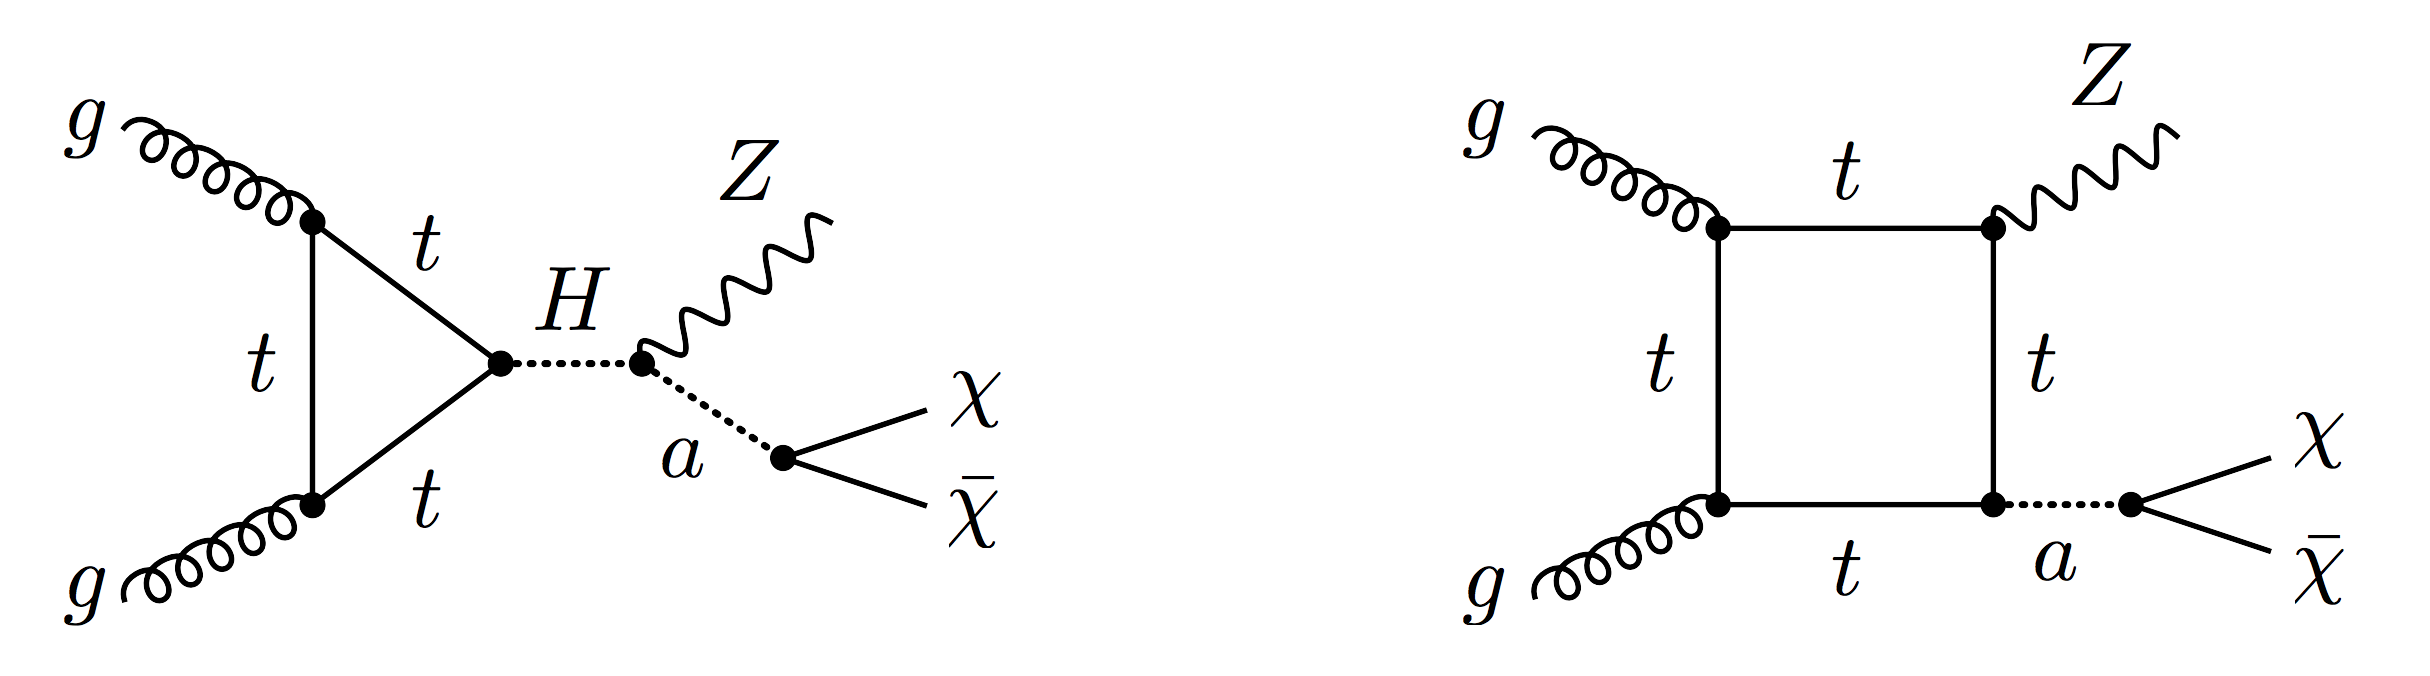
\includegraphics[width=0.75\textwidth]{Figures/2hdma.png}
\caption{2HDM+PS diagrams for the \monoZ signature produced by $gg$ fusion \cite{Bauer:2017ota}. The second diagram can have $A$ in place of $a$.}
\label{fig:2hdmaDiagrams}
\end{figure}

A popular model in Run 2 \monoX dark matter searches is known as the two Higgs doublet + pseudo-scalar (2HDM+PS) model \cite{Bauer:2017ota}. The addition of another SU(2) doublet to the SM is essential for many well-motivated BSM theories \cite{Branco:2011iw}. 2HDM models are also perturbative, and avoid violating unitarity by allowing mixing between the dark matter mediator and other bosons. 

Figure \ref{fig:2hdmaDiagrams} shows the two main diagrams of the 2HDM+PS model with the \monoZ signature. This model has two CP-even scalars $h$ and $H$ (where $h$ is the SM Higgs with $m_h$ = 125 GeV and $m_H > m_h$), one CP-odd pseudo-scalar $A$, two charged scalars $H^+$ and $H^-$, and the pseudo-scalar $a$ that couples the SM to dark matter. There are also the parameters $\sin(\beta-\alpha)$ and $\tan \beta$, where $\alpha$ is the mixing angle between $h$ and $H$, and $\tan \beta$ is the ratio of their vacuum expectation values. The parameters are chosen to have $m_A = m_H = m_{H^\pm}$.

Such models are of great interest to the \monoZ search because the \monoZ signature has better sensitivity than mono-jet for some regions of phase space. This is not the case for simplified models, where the mono-jet analysis always has higher sensitivity. In addition, there are couplings between $H$ and the $Z$ that are unique to the \monoZ search.

So far the \monoZ analysis has excluded a range of signals from the simplified and 2HDM+PS models. Prospective models to be studied with the full Run 2 dataset will be discussed in Chapter \ref{chapter:fullRun2}, including coloured scalar mediator ($t$-channel) signatures and so-called Less Simplified models.

\clearpage

% --------------------------------------------------------------------------------------
\section{The LHC and the ATLAS Detector}

The Large Hadron Collider (LHC) is the world's largest particle accelerator with a circumference of 27 km. Superconducting magnets are used to steer two beams of protons around the LHC as they are accelerated to nearly the speed of light. The beams are then brought to collision at various points around the LHC. Located at one of these collision points is the ATLAS detector, one of the two multipurpose detectors at the LHC. The LHC has been colliding protons at a centre-of-mass energy of 13 TeV since 2015, and ATLAS has been recording data.

The amount of \pp collision data delivered by the LHC is quantified by the \textit{luminosity}. The total number of $pp$ collisions $N$ detected over all time $t$ is related to the cross section for $pp$ collisions $\sigma$, and can be expressed in terms of either the instantaneous luminosity $L$ or the integrated luminosity $\mathcal{L}$:

\begin{equation}
N = \sigma \int{L} \text{d}t = \sigma \mathcal{L}
\end{equation}

\noindent $\mathcal{L}$ is the measure of total data collected that is frequently quoted in ATLAS. It has units of cm$^{-2}$, but a more frequently used unit is the inverse barn. 1 b = 10$^{-28}$ m$^2$. The total amount of data delivered by the LHC in the 2015-2017 period is 93 \ifb. ATLAS has recorded a total of 86 \ifb, with 80 \ifb that is good for physics analyses.

\begin{figure}[htb]
\centering
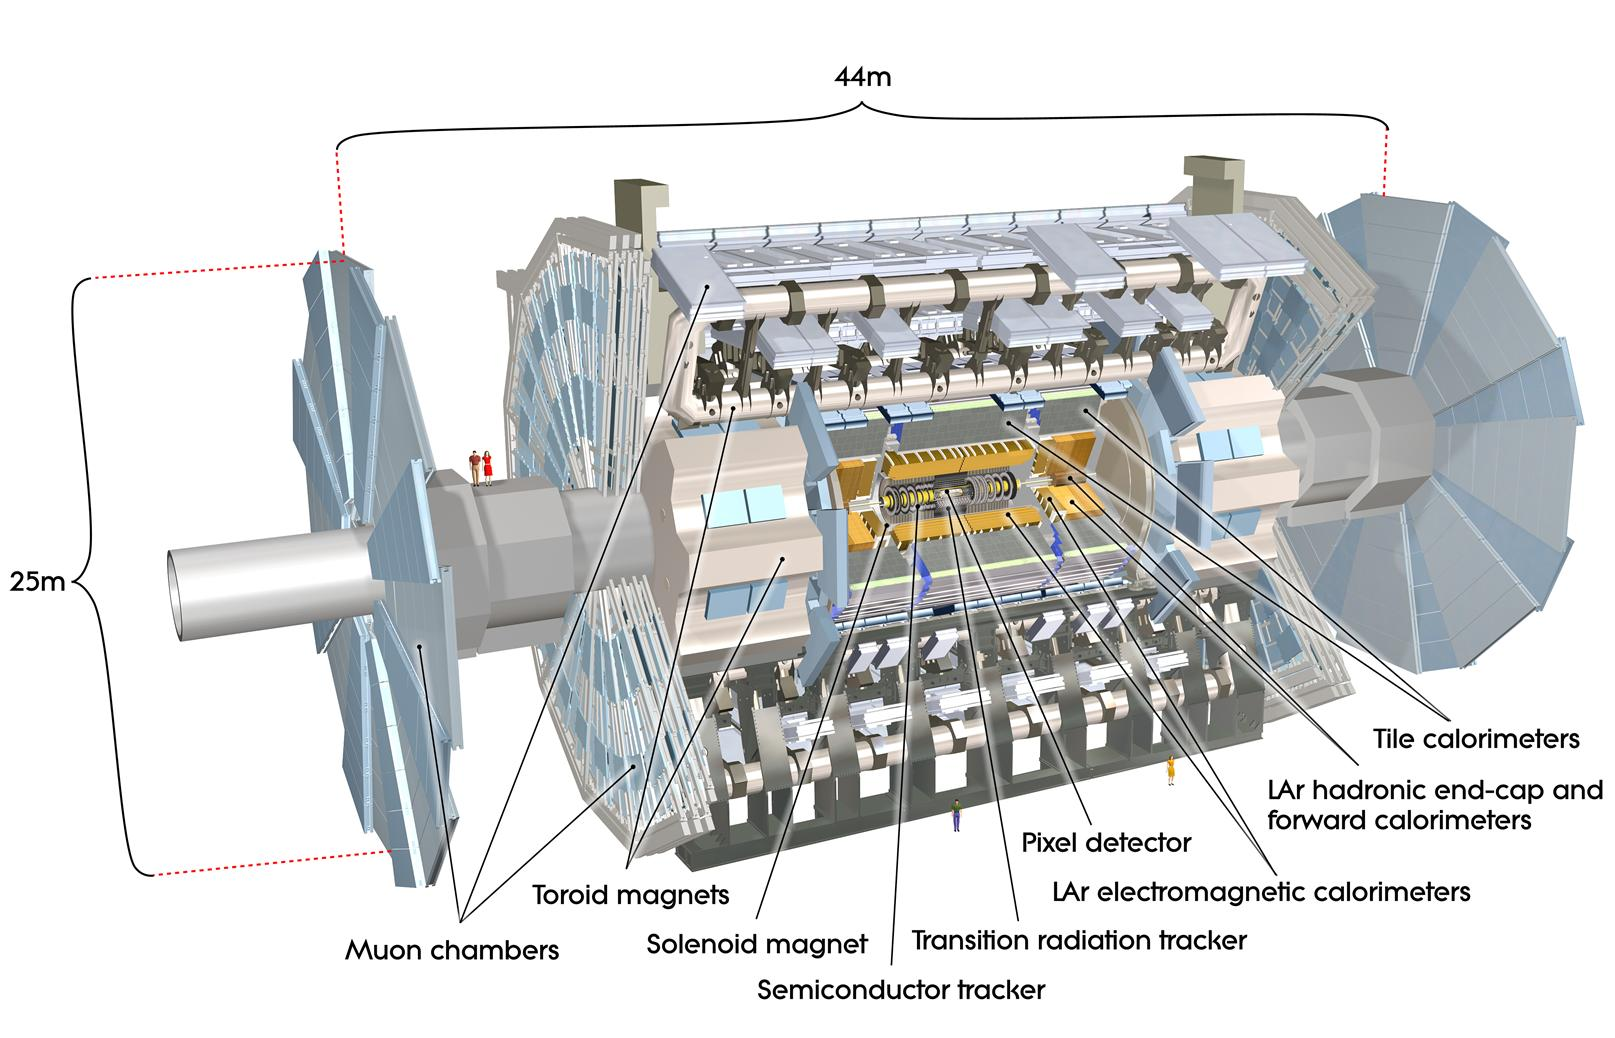
\includegraphics[width=1\textwidth]{Figures/atlas.jpg}
\caption{A cutaway view of the ATLAS detector with different subsystems labelled. The two humans on the left set the scale of the detector.}
\label{fig:atlas}
\end{figure}

An overview of the ATLAS detector is shown in Figure \ref{fig:atlas}. It is composed of four major subsystems. The innermost system is the inner detector which measures the tracks of charged particles very near to the collision point. It consists of three layers known as the pixel detector, semiconductor tracker, and transition radiation tracker. The innermost pixel detector has the highest resolution granularity in the detector and consists of 80 million pixels. The semiconductor tracker consists of 60 m$^2$ of silicon microstrips with densely packed readout channels, and the transition radiation tracker consists of 300,000 wires encased in straw tubes to measure tracks from ionization. The inner detector is encased in a solenoid that exerts a 2 Tesla magnetic field. The magnetic field causes the paths of charged particles to bend. The momentum of the particles can be determined from the curvature of the tracks.

Moving outward from the centre of the detector, the next subsystems are the electromagnetic and hadronic calorimeters. The electromagnetic system is entirely composed of liquid argon calorimetery, while the hadronic system includes the tile calorimeter in the barrel region and liquid argon calorimetry in the end-caps. The calorimeters are dense and designed to stop particles completely so that their energy is deposited entirely inside the detector. The electromagnetic calorimeter is designed to stop particles that interact electromagnetically (electrons and photons) while the hadronic calorimeter is designed to stop hadrons (e.g.\ protons and neutrons). The liquid argon calorimeter consists of alternating layers of copper absorber material and liquid argon ionization chambers, while the tile calorimeter alternates between layers of steel and plastic scintillators. 

The outermost and largest system of the detector is the muon spectrometer. Muons will interact minimally with the detector and so the spectrometer is designed to measure their momenta from tracks. The spectrometer consists of several systems. Monitored drift tubes are used in the barrel and end-caps for measuring track curvature. Resistive plate chambers, cathode strip chambers, and thin gap chambers are used for precision coordinate measurements throughout the spectrometer. The muon spectrometer also contains the ATLAS toroid magnet system.

Events that occur in the detector are recorded by the ATLAS trigger system. Due to the incredibly high rates of collisions inside the detector, it's not feasible to record every event that occurs (and most events are not interesting). The Level 1 trigger is hardware-based and makes decisions based on energy clusters in the calorimeter or coincidences in the muon spectrometer. If the event passes the Level 1 trigger, then it moves to the High Level Trigger, a more sophisticated software-based algorithm. A single electron trigger in the High Level Trigger may require, for example, that an object meets some electron identification criteria, has some minimum \pt, and is relatively isolated. The event is recorded to disk if the Level 1 and High Level Trigger selection criteria are satisfied.

\begin{figure}[!htb]
\centering
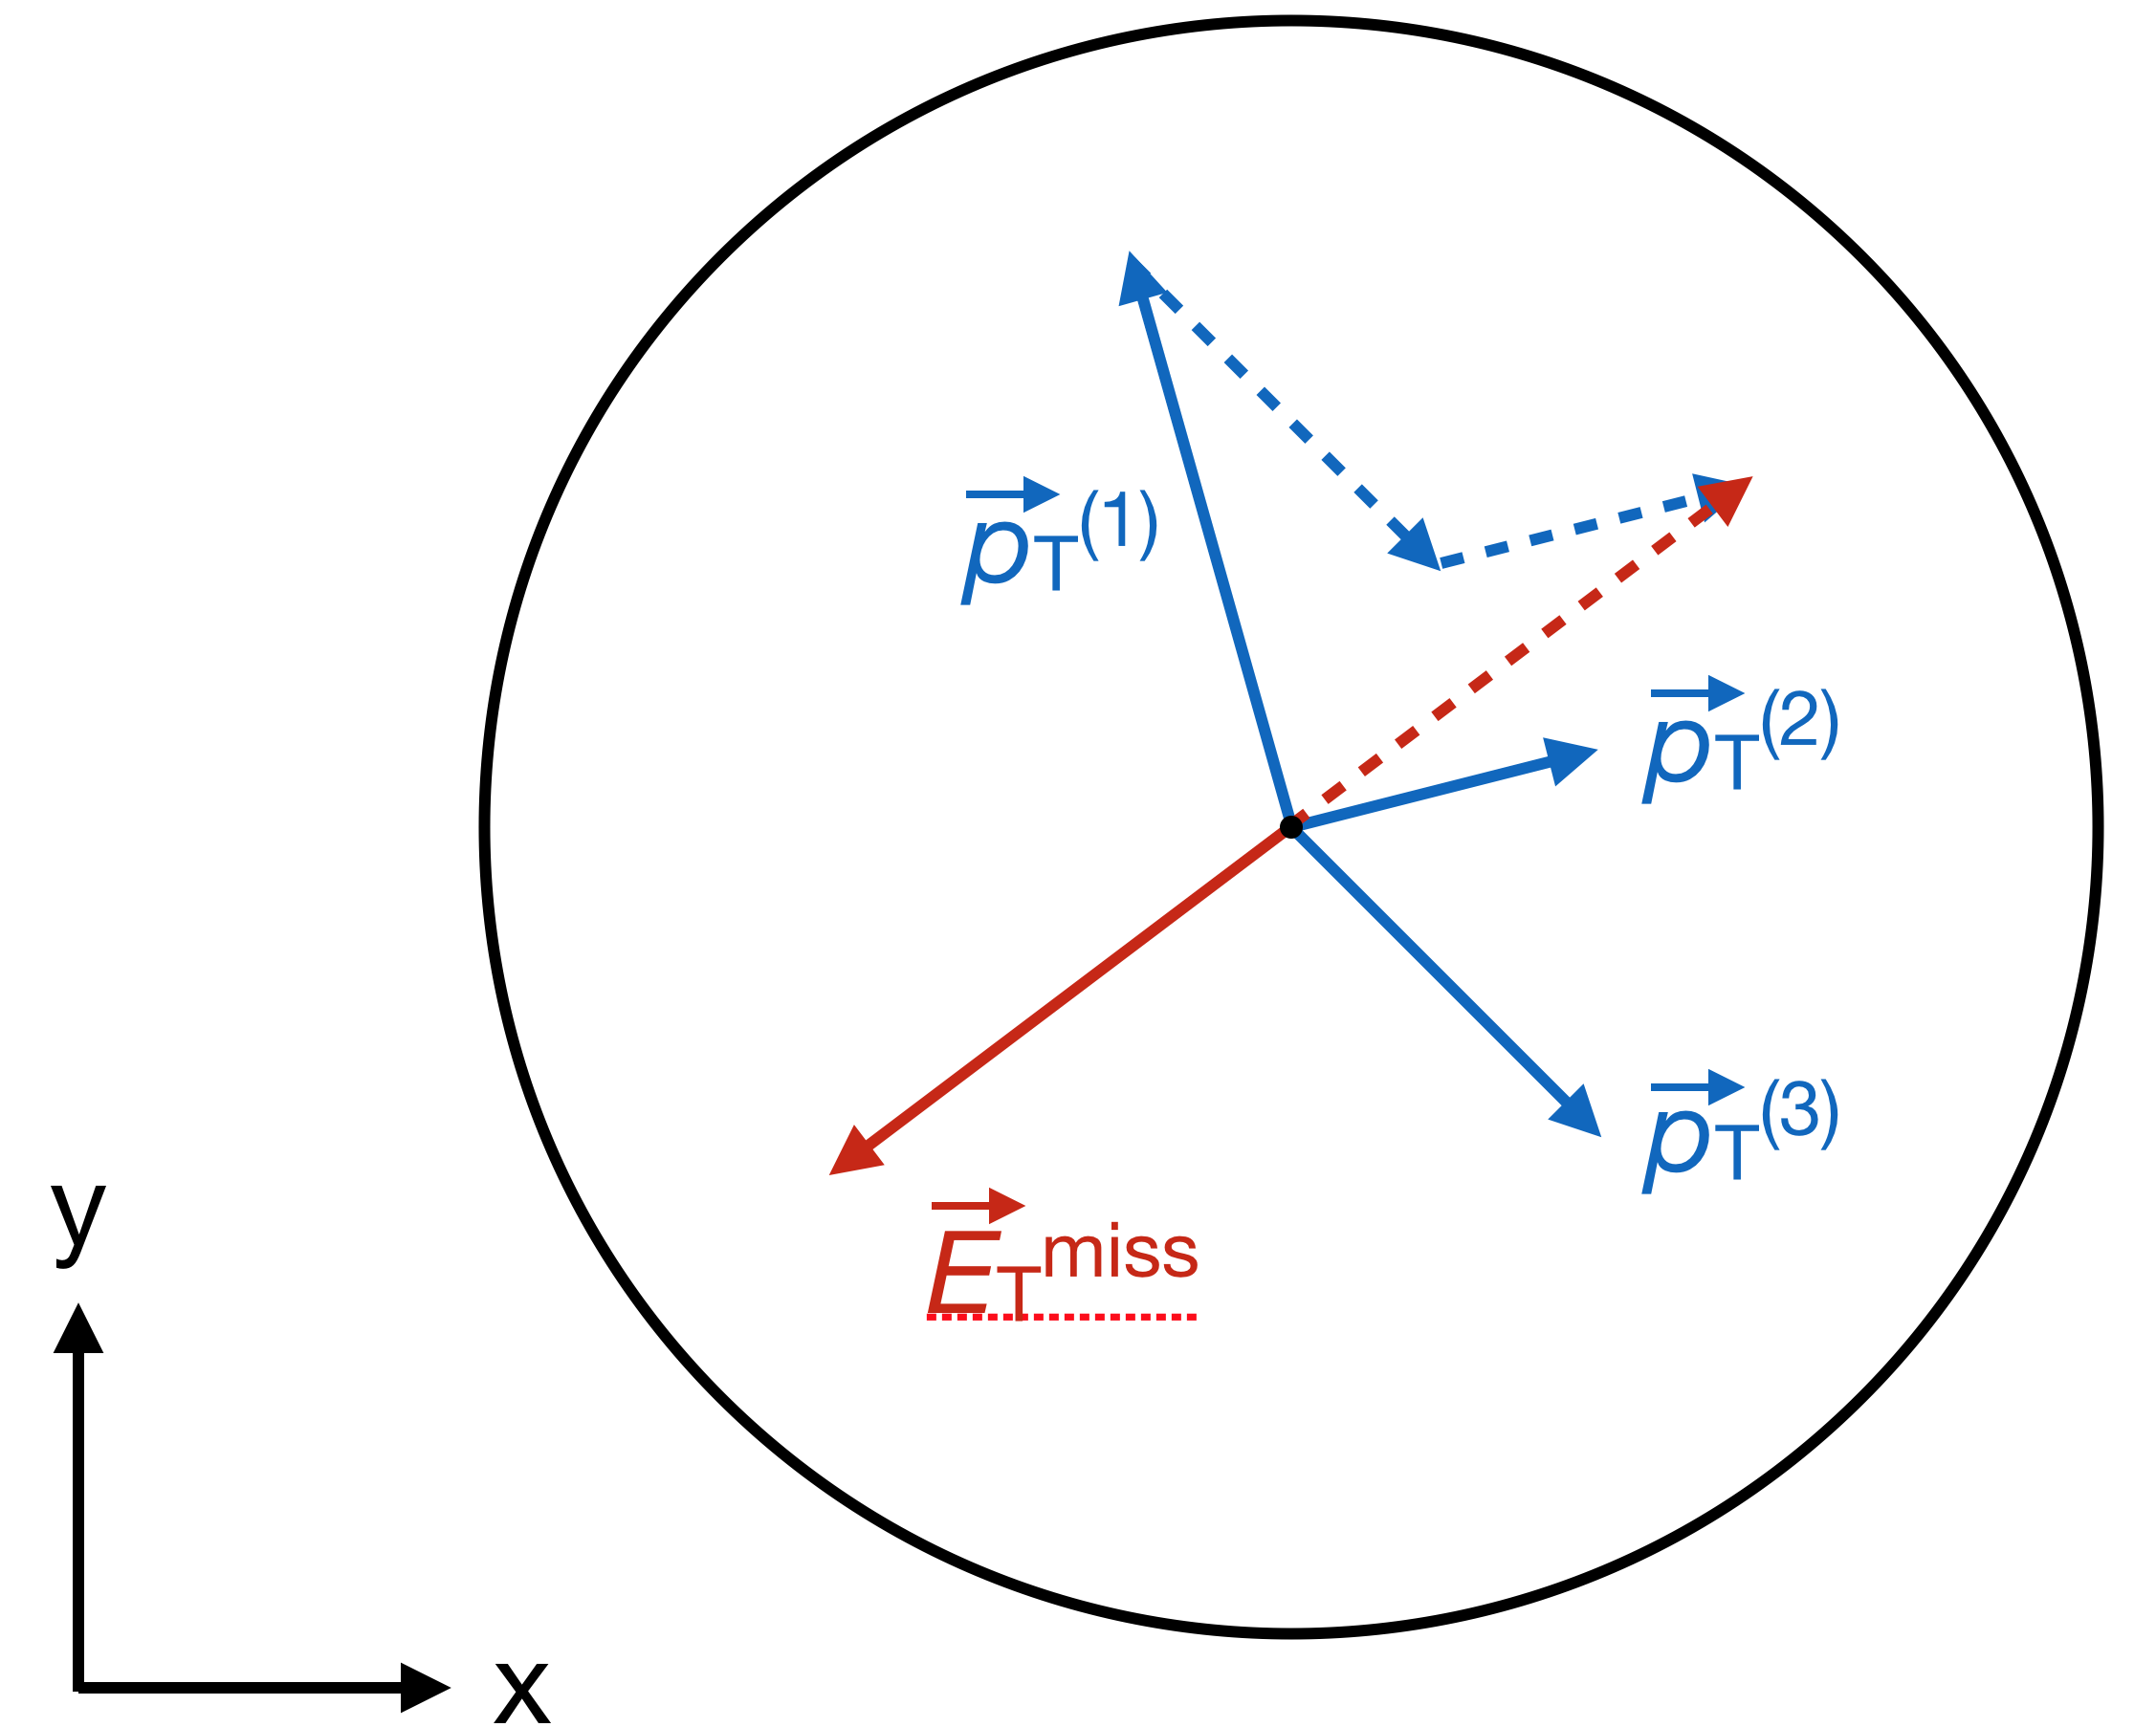
\includegraphics[width=0.4\textwidth]{Figures/etmiss.png}
\caption{Schematic of the missing transverse momentum \etmissvec.}
\label{fig:etmiss}
\end{figure}

Events that are recorded and deemed to be ``good for physics'' can be analyzed. The reconstructed objects in the events include electrons, photons, muons, and jets. The \etmiss is calculated using the reconstructed objects in the event. Figure \ref{fig:etmiss} shows an example of the transverse plane for an event with three measured particles. The \pt of the reconstructed objects in the event are added together (shown by the red dashed vector). Then the negative is taken to balance the measured \pt in the event (the solid red vector). This is the \etmissvec. The vector quantity \etmissvec is known as the missing transverse momentum, while its magnitude \etmiss is referred to as the missing transverse energy. The formal definition is given by:

\begin{equation}
\vec{E}_\text{T}^\text{miss} = - \left( \sum \vec{p}_\text{T}^\text{ jets} + \sum \vec{p}_\text{T}^\text{ electrons} + \sum \vec{p}_\text{T}^\text{ muons} + \sum \vec{p}_\text{T}^\text{ soft track} \right)
\end{equation}

\noindent The soft track term is formed from leftover tracks that are not used in reconstructed objects. Calorimeter energy clusters can also be used for this term, but tracks are more robust in high pileup environments. 

The physics objects used for a given analysis may have to satisfy further, stricter requirements, such as residing in a specific region of the detector. Then those selected objects are used to calculate the kinematic quantities used in the event selection.

\clearpage


	\startchapter{The \MonoZll Search}
\label{chapter:prevWork}

This chapter summarizes the previous work done. Section \ref{sec:analysis} gives an overview of the analysis, while Sections \ref{sec:truth} - \ref{sec:code} discuss specific contributions in more detail.

% --------------------------------------------------------------------------------------
\section{Analysis Overview}
\label{sec:analysis}

There are several important aspects of the \monoZ search. The analysis has been repeated fully twice during Run 2, once with the 2015 dataset (3.2 \ifb) and again with the 2015+2016 dataset (36.1 \ifb). The next result will not be ready until the full 2015-2018 Run 2 dataset is collected. The techniques discussed in this section are mainly based on the previous results from the 2015+2016 dataset. 

One of the the first steps of the analysis is to optimize the event selection for the specific signal being considered in the search. A \textit{signal region} must be chosen using some metric that optimizes the amount of signal compared to background. Background events are caused by SM processes that produce the same signature as the dark matter signal. Ideally such processes should be as suppressed as possible in the signal region. Event selections are optimized using Monte Carlo (MC) simulated events for signal and backgrounds. ATLAS MC are sophisticated and include effects from the detector, such as energy resolution. In general, events are selected in order to isolate a \epem or \mpmm pair that have an invariant mass close to the \Z and are recoiling against a sizeable \etmiss vector. The most important kinematic variables are identified and calculated using reconstructed objects as measured in the ATLAS detector (approximate in MC). Additional selection requirements are used to reduce background contributions while attempting to preserve signal. Two signal regions are used in the \monoZ analysis, one where \epem events are selected and the other where \mpmm events are selected.

Another crucial part of the analysis is in-situ background estimation. Once a signal region has been defined, data can then be used to estimate the dominant backgrounds in that region. When possible it is always preferable to use data instead of MC estimations. This is typically done by defining a control region that has a very high purity in background events, and then somehow transferring the estimate into the signal region. The major backgrounds in the analysis are described below with their percent contribution from the 2015+2016 result. They all emulate the signal by producing $\ell\ell+E_{T}^\text{miss}$. All backgrounds except for the $ZZ$ background are estimated from data.
\begin{enumerate}
	\item	 $ZZ \rightarrow \ell \ell \nu \nu$ (56\%): Dominant, irreducible background. Estimated entirely with MC. 
	\item	 $WZ \rightarrow \ell \nu \ell \ell$ (27\%): Lepton from the $W$ is not reconstructed. 
	\item \Zjets (8\%): Jet(s) are mis-measured as fake \etmiss. 
	\item $WW$, $Wt$, $t\bar{t}$, and $Z\rightarrow \tau \tau$ (8\%): Lepton pair does not come from a \Z.
	\item $W$+jets ($<1\%$): Lepton is misidentified from a jet.
\end{enumerate}

\noindent The data-driven estimation techniques for each of the backgrounds are complex and are not discussed in detail here. Previous work on the estimation of the \Zjets background is discussed ahead.

There are several sources of systematic errors that must be considered in any ATLAS analysis. Experimental systematics come from detector effects, such as the uncertainty in identifying an electron, energy uncertainties due to resolution effects, etc. These systematics are applied to MC samples. Data-driven background estimates will have systematic errors associated with the specific estimation technique. These types of systematics are often the dominant source of systematic uncertainties. Finally, there are theoretical systematics associated with the simulated dark matter signal, including errors from QCD, PDF, and parton showering effects. These will be discussed in more detail in the following section.

\begin{figure}[htb]
\centering
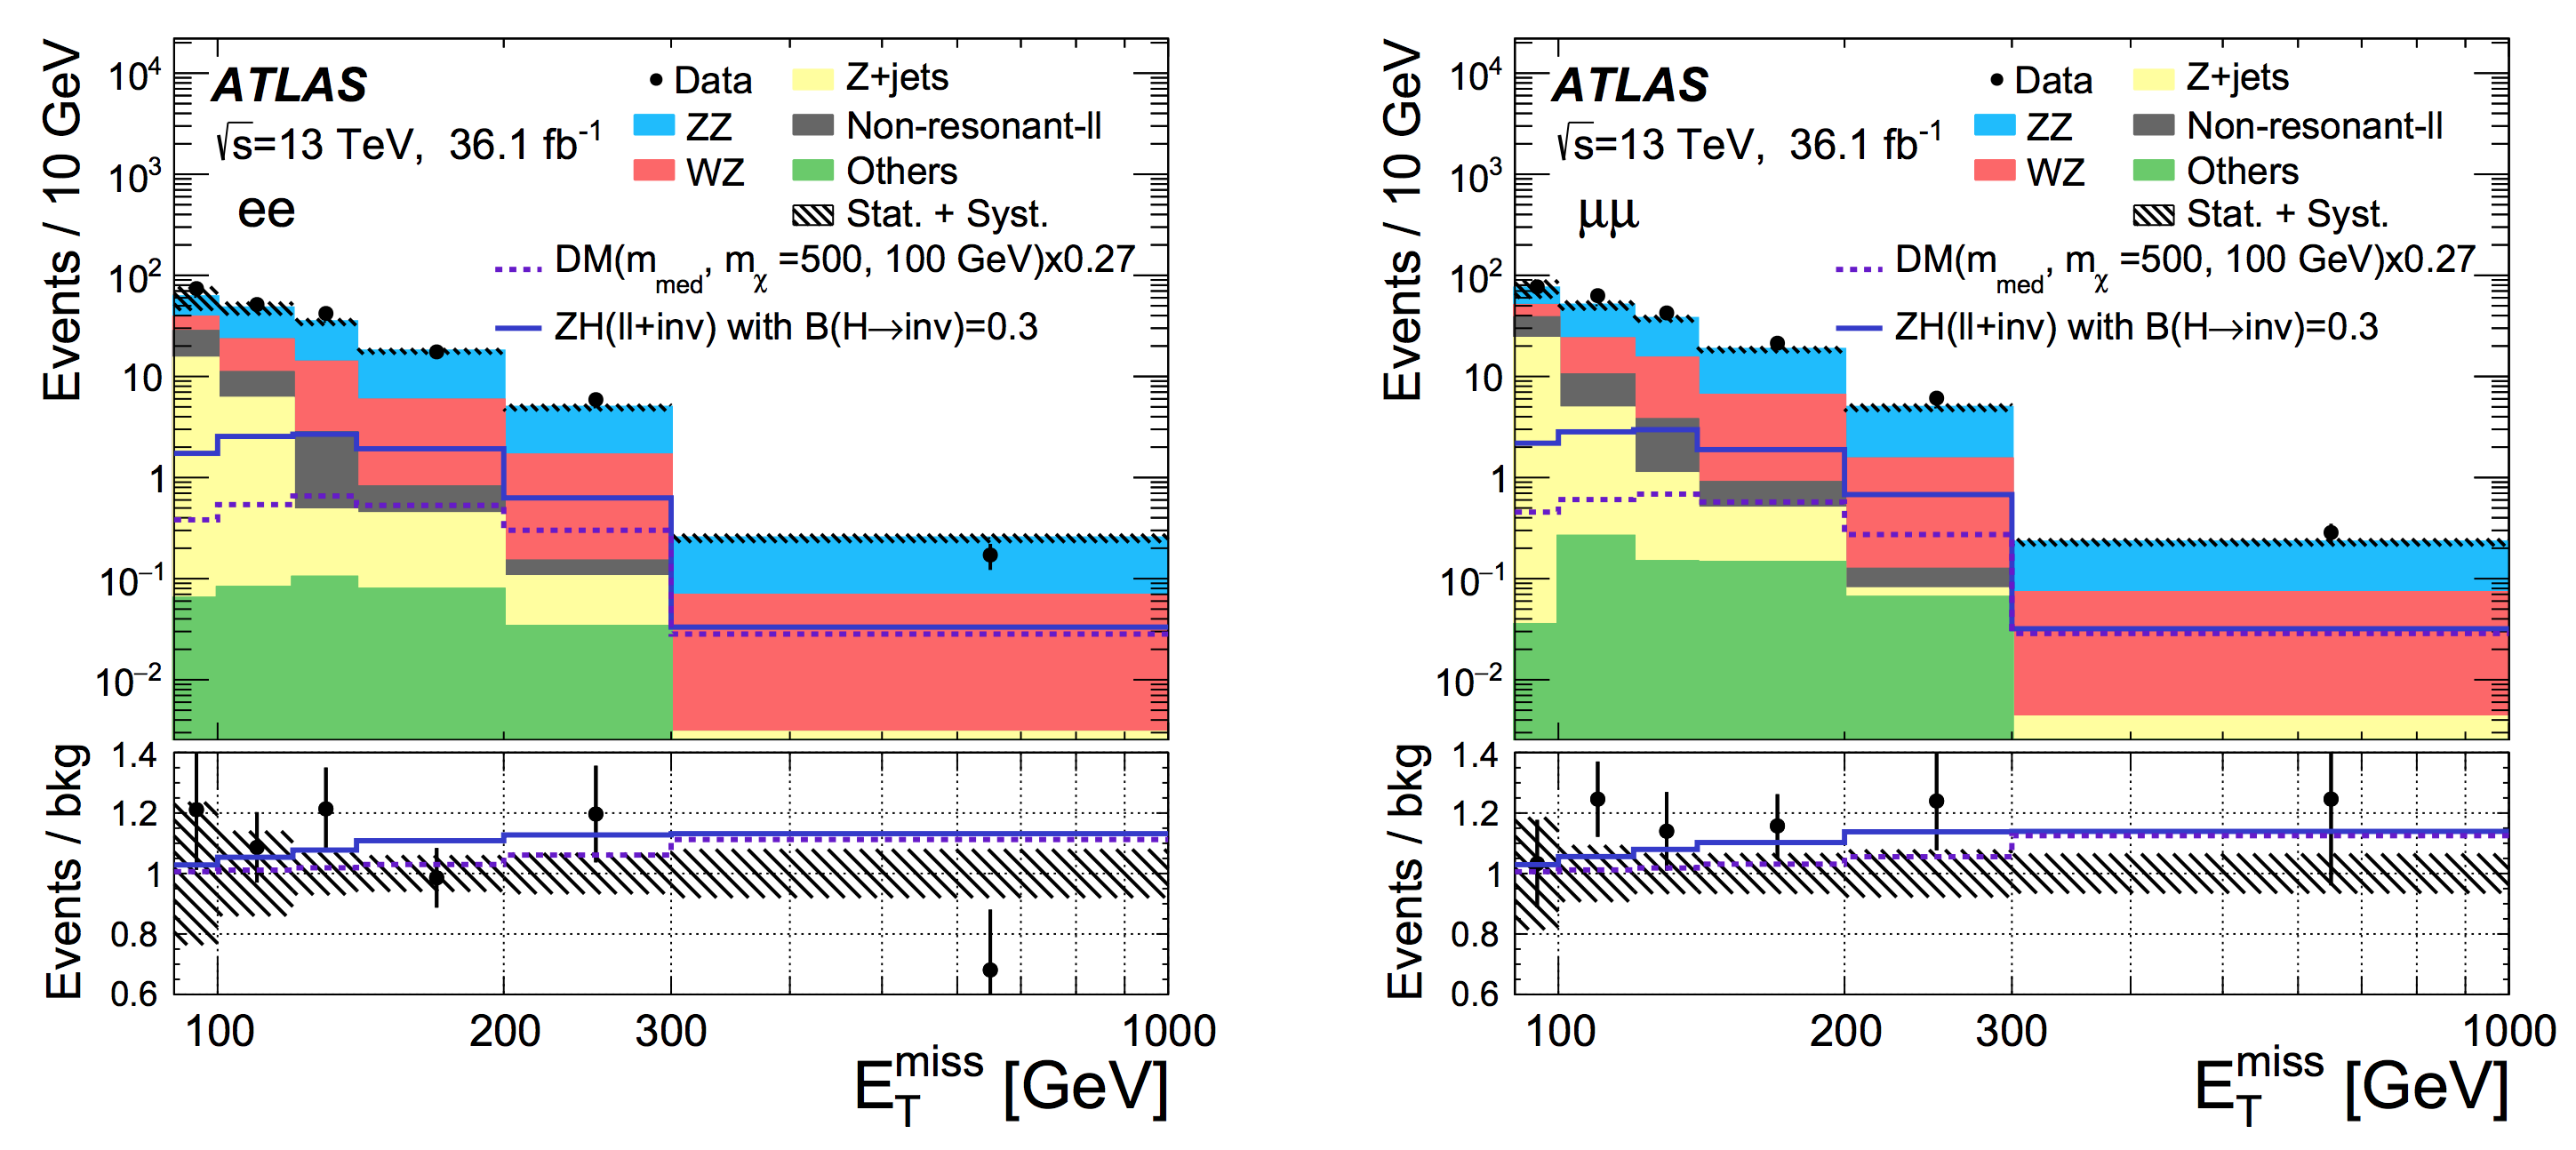
\includegraphics[width=1\textwidth]{Figures/srEPS.png}
\caption{Text}
\label{fig:srEPS}
\end{figure}

After defining a signal region, estimating backgrounds in that signal region, and accounting for the systematic uncertainties of the analysis, the signal region is \textit{unblinded} and the agreement between observed data and expected background estimates is quantified. In the \monoZ analysis the \etmiss is the distribution of interest, where a dark matter signal could manifest. The signal region \etmiss distributions from the 2015+2016 analysis are shown in Figure \ref{fig:srEPS}. If an excess in data is found then there is potential for a discovery. However, as in past iterations of the analysis, if no excess is seen then limits can be set on the dark matter model being studied. This is discussed in detail in the final section of this chapter.

% --------------------------------------------------------------------------------------
\section{Truth Studies} 
\label{sec:truth}

Truth studies are often useful when we want to ignore the effects of the ATLAS detector. \textit{Reconstructed} MC samples include simulation of the detector, whereas \textit{truth-level} MC samples come directly from the MC generator, typically \textsc{MadGraph}. Studying these samples allow us to study theoretical effects on the signal. In addition, such samples can be produced quickly and locally, whereas reconstructed samples must undergo heavy duty ATLAS reconstruction which can be computationally intensive. 

A framework has been adapted, called MonoZTruthUVic, for applying truth-equivalent analysis cuts to truth samples. This allows for the analysis to be reproduced at the truth-level. This is useful for several reasons and allows us to estimate how many signal events are theoretically predicted to be in the signal region.

An important study that must be performed at the truth-level is the estimation of theoretical uncertainties on the signal \textit{acceptance}, the number of signal events that end up in the signal regio. There are potentially significant sources of systematic uncertainties from theory that must be considered. It should be noted that systematics from uncertainties in the parton distribution function (PDF) are evaluated in the analysis but are not discussed in detail here. 

The signal acceptance depends on two scales from quantum chromodynamics (QCD) known as the renormalization and factorization scales, $\mu_r$ and $\mu_f$. Both scales are arbitrary and arise from finite order perturbation theory. $\mu_r$ is related to the renormalization of ultraviolet divergences, and $\mu_f$ qualitatively corresponds to the resolution at which the proton is being probed. The cross section for some hard process depends on these scales via

\begin{equation}
\sigma = \int \text{d}x_1 \text{d}x_2 f_1(x_1, \mu_f^2) f_2 (x_2, \mu_f^2) \hat{\sigma}(x_1 p_1, x_2 p_2, \alpha_s(\mu_r), Q^2, \mu_r^2, \mu_f^2),
\end{equation}

\noindent where partons 1 and 2 have PDFs $f_1$ and $f_2$ and momentum fractions $x_1 p_1$ and $x_2 p_2$ respectively. $Q$ is the scale of the hard scatter process determined by the cross section $\hat{\sigma}$.
In short, by simulating dark matter MC with different values for $\mu_f$ and $\mu_r$ and then applying truth-level analysis cuts, the systematic error on the acceptance due to the choice of scales can be quantified. The convention is to generate two variational samples with $\mu_r = \mu_f$, where the scales are doubled in one sample and halved in the other. Then the signal acceptance for both variational samples is calculated and compared to the nominal acceptance. The largest change is taken as the systematic error. This systematic has been observed to be independent of $m_{DM}$, so the errors are evaluated as a function of \mmed. An example of the errors previously used for axial-vector signals is illustrated in Figure \ref{fig:qcd}. These errors are on the order of 1-2\%.

\begin{figure}[htb]
\centering
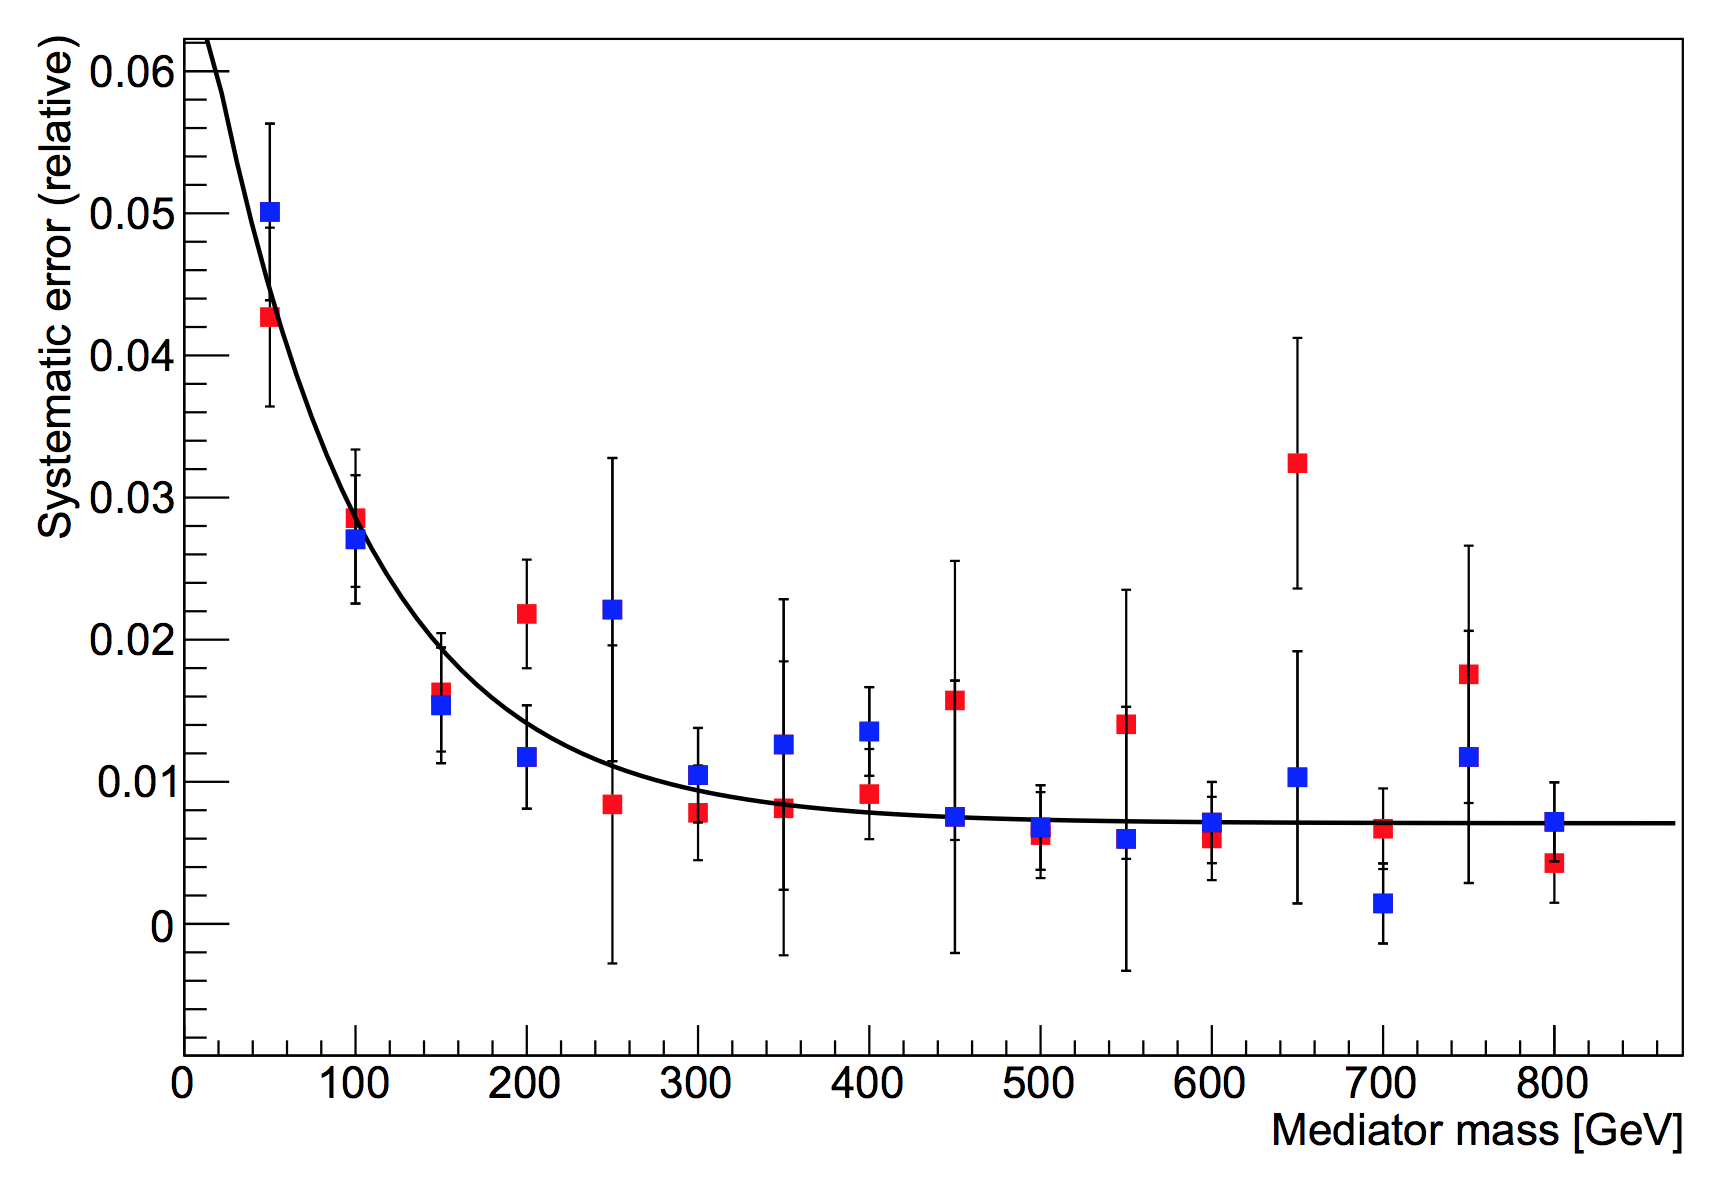
\includegraphics[width=0.5\textwidth]{Figures/qcd.png}
\caption{QCD scale uncertainties as a function of mediator mass for axial-vector signals. Red and blue points correspond to errors obtained from the \ee and \mm signal regions respectively.}
\label{fig:qcd}
\end{figure}

The other source of theoretical uncertainty on the signal acceptance comes from parton showering effects. In the MC samples used by ATLAS, after the hard scatter is simulated it is run through a showering simulator called \pythia. \pythia adds in several physical effects such as the underlying event (UE), initial and final state radiation (ISR and FSR) of extra jets, and multiple parton interactions (MPI). These are complicated processes governed by QCD and the number of parameters in \pythia that can be set are extensive. To simplify this, ATLAS has a standardized \pythia \textit{tune}, i.e. a set of parameters that serve as the default to be used in MC showering. The signal acceptance depends on the choice of this tune. The uncertainty is evaluated using a prescription whereby ten variations are used to account for each general effect. As for the QCD scale uncertainties, variational MC samples are produced according to each variation, and the difference in the signal acceptance is evaluated compared to the nominal showering. These systematics are typically on the order of 5\%.


% --------------------------------------------------------------------------------------
\section{Estimation of the \Zjets Background}
\label{sec:zjets}

% -------------------------------------------
\subsection{ABCD Method}

\begin{figure}[htb]
\centering
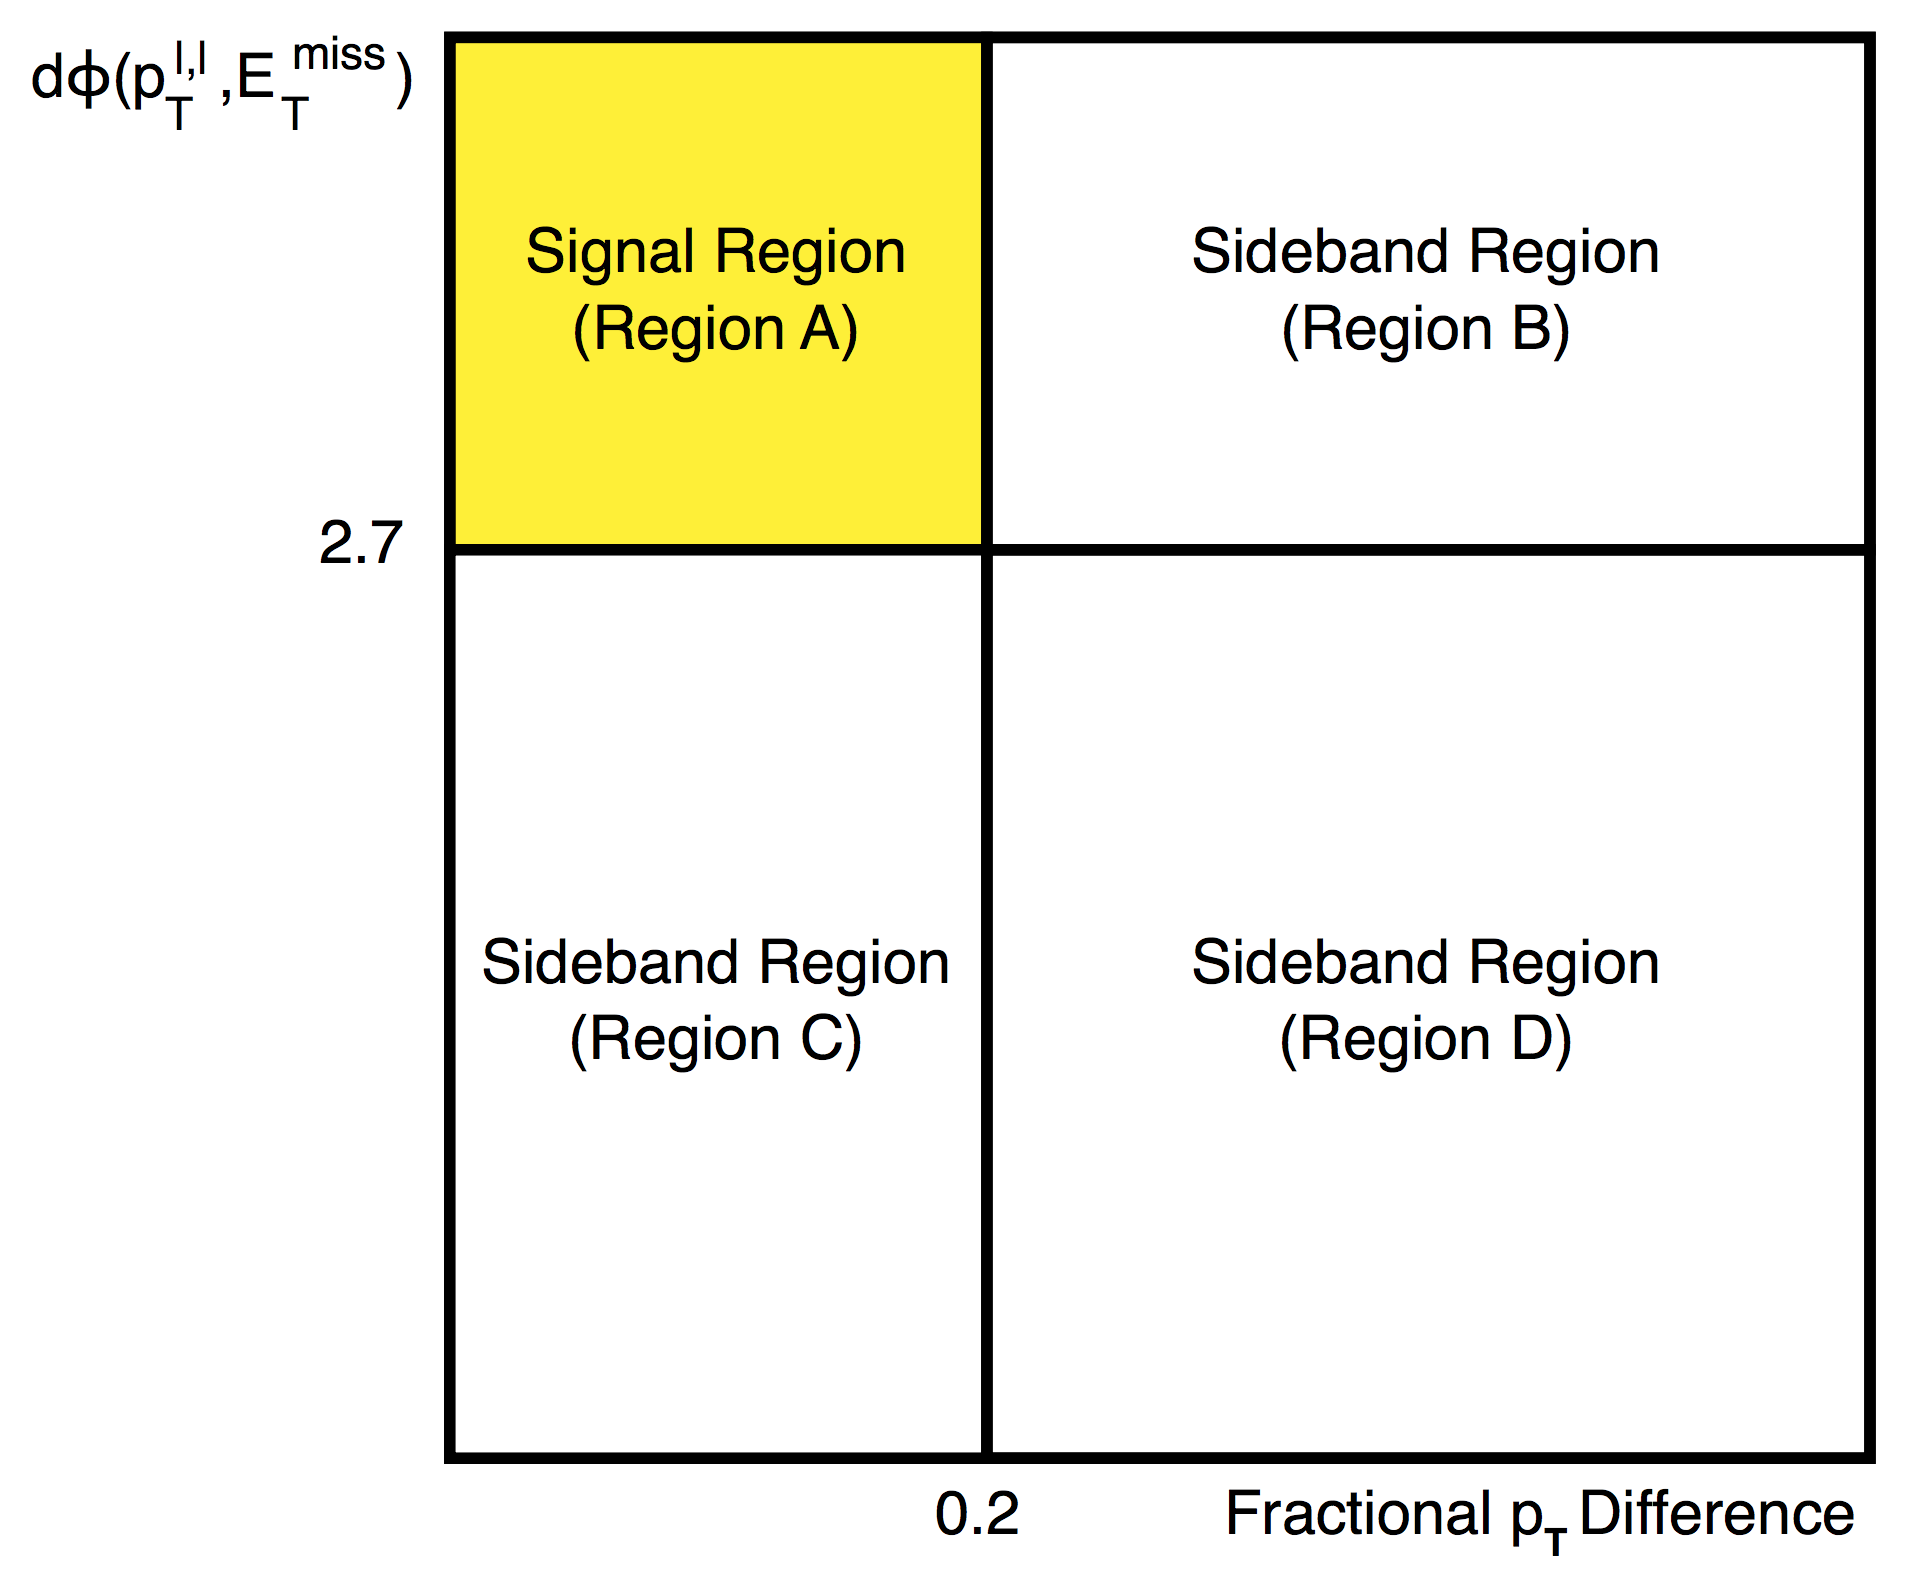
\includegraphics[width=0.5\textwidth]{Figures/abcd2.png}
\caption{Scheme of the ABCD method.}
\label{fig:abcd}
\end{figure}

One data-driven technique for estimating the \Zjets background is the ABCD method. This was the primary estimation method used for the 2015 result. A schematic of the method is shown in Figure \ref{fig:abcd}. Four regions are defined using two of the kinematic variables from the event selection. This pair of variables is chosen to optimize event statistics in the sideband regions (B, C, and D) and to minimize the correlation between them. Region A is the signal region, the target region that we are trying to estimate the background in. The number of background events in the sidebands are used to estimate the number of background events in A using the assumption that $N_A/N_C = N_B/N_D$. This is true if there is no correlation between the two variables. Then the number of \Zjets events in A is given by:

\begin{equation}
N_\text{A}^\text{est} = N_\text{C}^\text{obs,corr} \times \frac{N_\text{B}^\text{obs,corr}}{N_\text{D}^\text{obs,corr}}
\end{equation}

\noindent $N_\text{B}$, $N_\text{C}$, and $N_\text{D}$ are the observed number of events in each sideband control region with non-\Zjets events subtracted (using MC).

The main challenges for this method come from having correlations between the two variables and having enough statistics in data in all of the sidebands. The validity of this technique is evaluated by looking at the agreement between the three ratios $N_\text{A}/N_\text{C}$ (MC), $N_\text{B}/N_\text{D}$ (MC), and $N_\text{B}/N_\text{D}$ (data). If the method works perfectly then these ratios will agree. In addition, the agreement of these ratios should agree as the other event selections are applied. However, correlations cause deviations in the agreement, and low statistics in one or more of the sidebands can lead to large errors on the ratios after all selections are applied. And, if the ratios change with other selections, this suggests more complicated correlations with other variables that enhance the correlation between the two variables used for the method. These effects are all taken into account with systematic errors that are evaluated to be about $\pm$70\% on the \Zjets estimate. These turned out to be dominant uncertainties in the analysis for the 2015 result.

% -------------------------------------------
\subsection{\gjets Technique}

The \Zjets estimation had to be modified for the 2015+2016 result. The event selection was reoptimized and introduced new variables, and correlations had a more pronounced effect in the ABCD method. Because of this, a second technique was developed alongside a modified ABCD method. The technique is known as the \gjets reweighting method. The theory is described in \cite{Ask:2011xf} and the application has been adapted from an ATLAS SUSY search \cite{Galster:2151990}.

The \gjets method uses events with a photon and jets to estimate the fake \etmiss in \Zjets events. \gjets event topologies are similar to \Zjets events as they both consist of a well-measured \Z or photon recoiling against jets, and the \etmiss arises from jet mis-measurements. However there are some kinematic differences that need to be accounted for. This is done by reweighting the \gjets MC events to transport them to \Zjets MC events. Typically the \pt distribution of the photon is scaled to match the \pt distribution of the \Z (i.e. the \pt of the two leptons). The multiplicative factor needed to scale each \pt bin is used as an event weight for the \gjets events: 

\begin{equation}
w(p_\text{T}^\gamma) = \frac{N_{Z\text{+jets}}(p_\text{T}^{\ell\ell})}{N_{\gamma\text{+jets}}(p_\text{T}^\gamma)}
\end{equation}

\noindent After the reweighting the \etmiss distribution for the \gjets events improves to match the \Zjets events (most obviously the tail increases at high \etmiss). The reweighting is applied fairly early in the event selection and then subsequent selections are applied; the agreement between \gjets and \Zjets events is monitored down to the signal region. Once reliable agreement is seen, then the method can be performed using data instead of MC.

In the \monoZ analysis, \pt reweighting was not sufficient to have good agreement between \gjets and \Zjets events. Two approaches were taken in an attempt to rectify the remaining differences. The first is a photon smearing method as used in \cite{Galster:2151990}. This is done by looking at the component of the \etmiss along the \Z/photon direction, \etmisspar. The idea is that any difference in \etmisspar between \Zjets and \gjets events comes from lepton mis-measurements in the \Zjets events, leading to a larger \Z resolution compared to the photon. Hence the photon \pt and \etmisspar can be smeared to match the \Z resolution. This procedure was carried out in the \monoZ analysis but minimal improvements were seen because the photon and \Z were observed to have very similar resolutions. Therefore a second reweighting scheme was adapted to improve the agreement in the \etmiss distributions. Instead of only reweighting by \pt, a secondary reweighting is applied using another variable. Several variables were investigated; in the end \etmissht gave the best results ($H_T$ = scalar sum of lepton \pt and jet \pt). In addition, the reweighting could be applied using 2D weights or with two 1D (2x1D) weights. The 2D reweightings that were investigated gave the best \etmiss agreement, but the weights were unreliable due to limited statistics (e.g. weights in \pt and \etmissht bins). 2x1D reweighting schemes were also studied. Here an added complication is that the two variables that are reweighted are treated as uncorrelated, whereas for 2D reweighting the correlation is accounted for automatically. So in a 2x1D scheme, when reweighting the second variable, if the previously reweighted \pt distribution does not change, then the variables can be treated uncorrelated. This was seen in \pt and \etmissht. Also the weights with 2x1D schemes were observed to be far more reliable because of the higher statistics use in the weight calculation. This was further tested by splitting the \gjets MC into two statistically independent halves; one half was used to obtain the weights and the other half had them applied. The agreement between both reweighted halves of the \gjets sample was excellent. 

\begin{figure}[h]
\centering
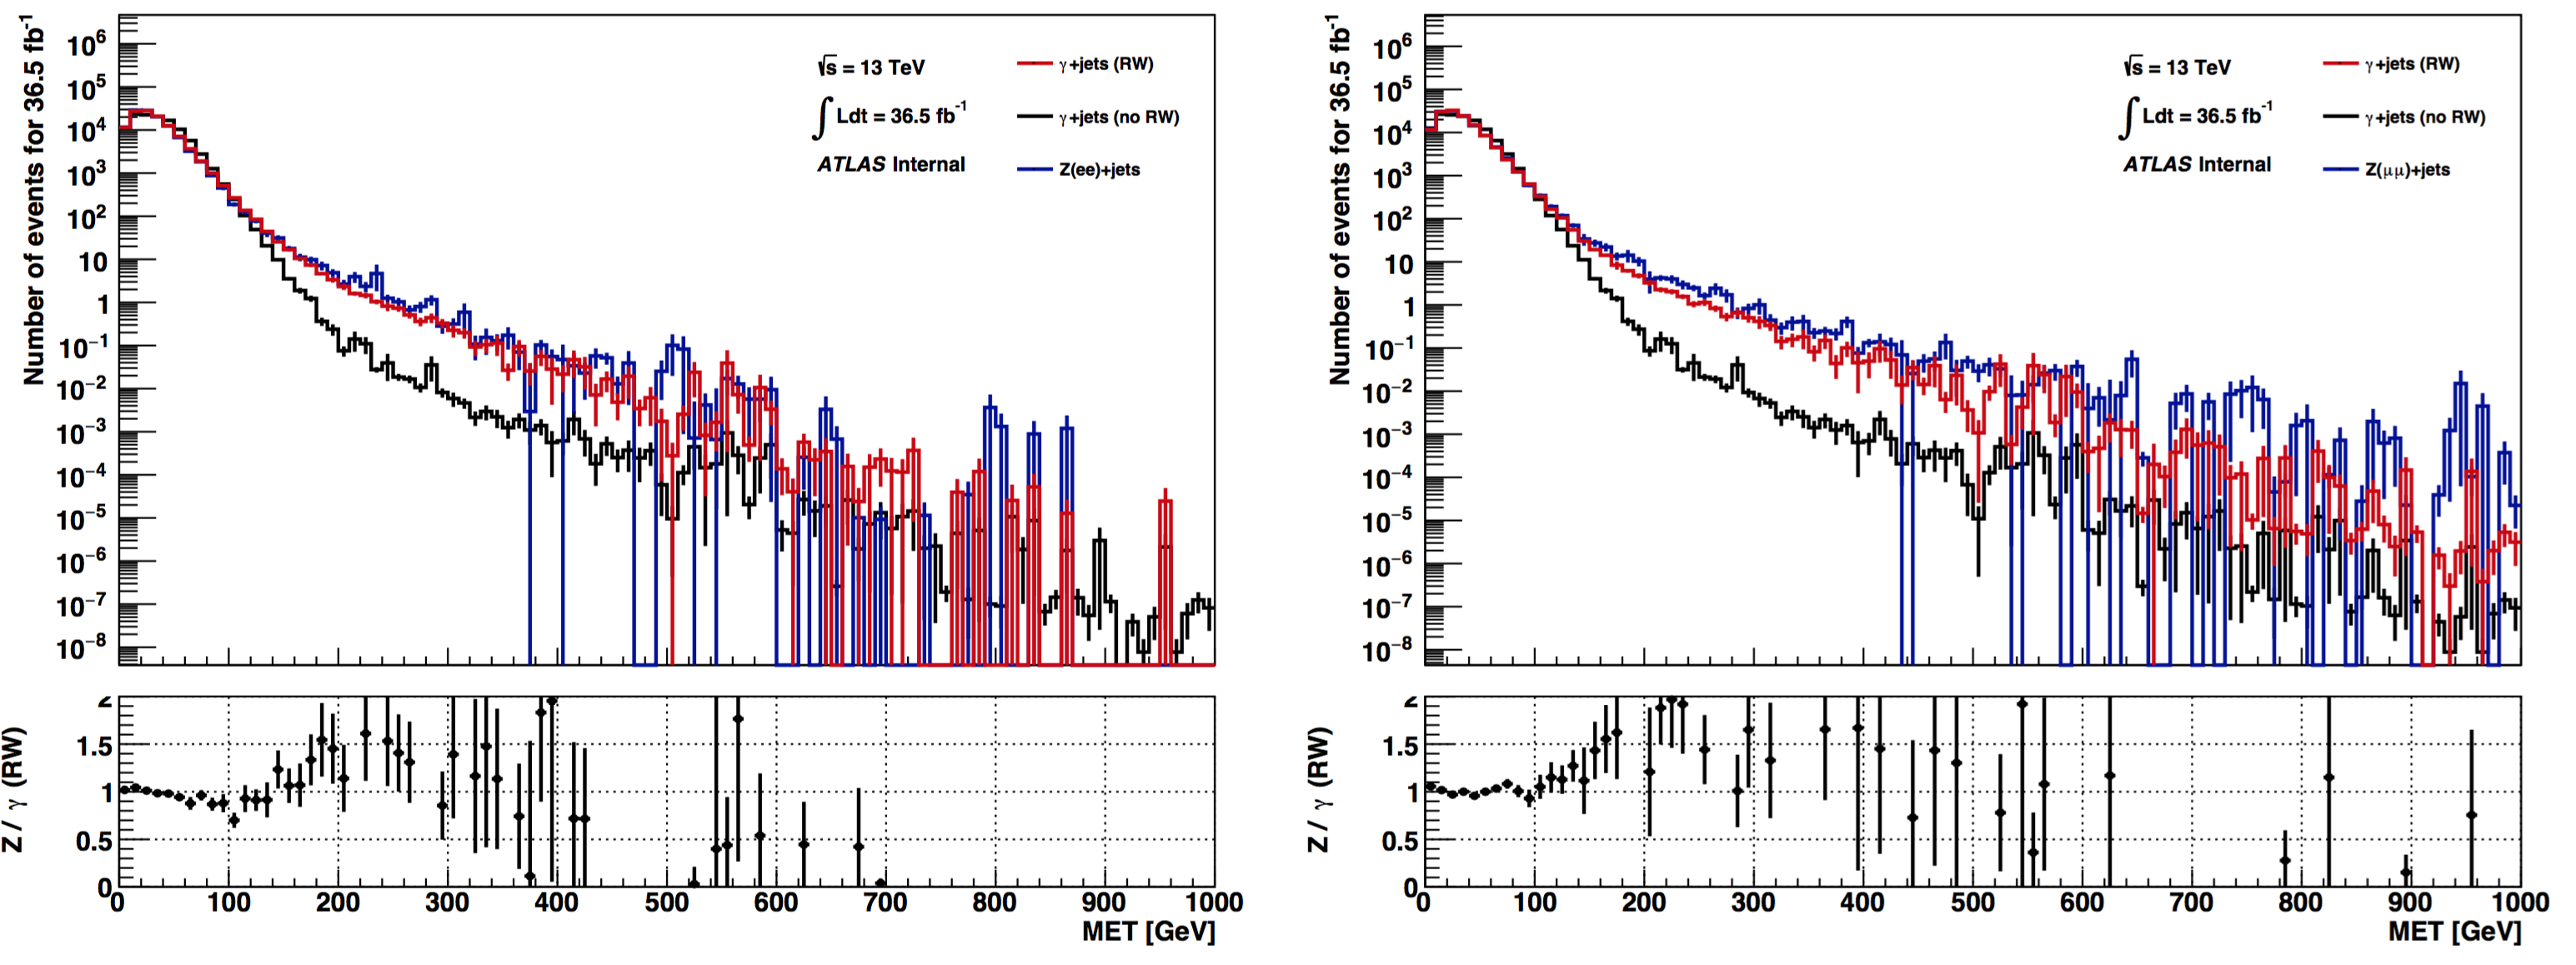
\includegraphics[width=1\textwidth]{Figures/gjets.png}
% EPS paper: https://arxiv.org/abs/1708.09624
\caption{\etmiss distributions for \gjets events (red) and \Zjets events (black without reweighting, blue with reweighting).}
\label{fig:gjets}
\end{figure}

Due to time constraints in the analysis for the 2015+2016 result, the development of this technique is still under development and has yet to be tested on data. In the end a 2x1D reweighting scheme using \pt and \etmissht gave the best results in MC. Figure \ref{fig:gjets} shows the \etmiss distributions for \Zjets and reweighted \gjets events (at an early selection step). From \Zjets MC, the predicted yield in the \ee and \mm signal regions is approximately $0.45 \pm 0.90$ events. The best observed reweighted \gjets prediction is $2.0 \pm 0.1$. The results nearly agree within statistical errors, but differences are still observed in the \etmiss tail. Since this is the region of interest in the \monoZ search, care must be taken to study these differences and quantify the systematic errors from the reweighting technique. The next steps to developing and improving the \gjets technique are discussed in the next chapter.

% --------------------------------------------------------------------------------------
\section{Dark Matter Limit Setting}
\label{sec:limits}

In the case that no excess is observed in data, upper limits are set on the signal strength for each of the dark matter models. These are then translated into limits on the masses of the dark matter particles, \mchi and \mmed. Hypothesis tests are performed using HistFitter. The signal region \etmiss distributions are inputted to HistFitter for signal, backgrounds, and all systematic uncertainties (also known as nuisance parameters or NPs). HistFitter calculates upper limits using the CL$_{s}$ method~\cite{Cowan:2010js}, a standard in the ATLAS experiment. 

The statistical analysis of the data uses a binned likelihood function constructed as the product of Poisson probability terms,
\begin{equation}
\mathcal{L} = 
\text{Pois}(n|\mu s+b)\left[\prod_{b\in \text{bins}}^{n}
\frac{\mu \nu_{b}^{\text{sig}} + \nu_{b}^{\text{bkg}}}{\mu s+b} \right],
\end{equation}
where $\mu$, the signal strength parameter, multiplies the expected signal yield $\nu_{b}^{\text{sig}}$ in each histogram bin $b$, and $\nu_{b}^{\text{bkg}}$ represents the background content for bin $b$. The dependence of the signal and background predictions on the systematic uncertainties is described by a set of NPs $\vec{\theta}$, which are each parametrized by a Gaussian. 

The nominal fit result is obtained by maximizing the likelihood function with respect to all parameters. This is referred to as the maximized log-likelihood, $\mathcal{L}(\hat{\mu}, \hat{\boldsymbol{\theta}})$, where $\hat\mu$ and $\hat{\boldsymbol{\theta}}$ are the parameters that maximize the likelihood. The test statistic $\tilde q_\mu$ is then constructed based on the profile likelihood ratio:

\begin{equation}
\lambda(\mu) = \frac{\mathcal{L}(\mu, \hat{\hat{\boldsymbol{\theta}}})}{\mathcal{L}(\hat{\mu}, \hat{\boldsymbol{\theta}})}
\label{eqn:proflike}
\end{equation}

\noindent $\hat{\hat{\boldsymbol{\theta}}}$ are the nuisance parameter values that maximize the likelihood for a given $\mu$. The level of compatibility is quantified using $\tilde q_\mu$, since larger values are interpreted as greater incompatibility between data and the assumed signal+background ($\mu=1$) hypothesis. The corresponding p-value, $p_\mu$, is defined as:

\begin{equation}
p_\mu = \int_{\tilde{q}_{\mu,\text{obs}}}^\infty f(\tilde{q}_\mu | \mu) \text{d}\tilde{q}_\mu
\label{eqn:pmu}
\end{equation}

\noindent Here $f(\tilde{q}_\mu | \mu)$ is the probability density function of $\tilde{q}_\mu$ assuming the $\mu$ hypothesis, and $\tilde{q}_{\mu,\text{obs}}$ is the value of $\tilde{q}_\mu$ computed for the observed data.
Asymptotic formulae~\cite{Cowan:2010js} are used to calculate the closed form for $f(\tilde{q}_\mu | \mu)$. $p_\mu$ can also be written as:

\begin{equation}
p_\mu \equiv p_{s+b} = P(\tilde q_\mu \geq \tilde{q}_{\mu,\text{obs}} | s+b)
\end{equation}

\noindent Performing exclusion tests with $p_{s+b}$ is known as the CL$_{s+b}$ method. This analysis uses the CL$_s$ method, where the p-value, or the ``CL$_s$ value,'' is defined as:

\begin{equation}
\text{CL}_s \equiv \frac{p_{s+b}}{1-p_b},
\end{equation}

\noindent where 

\begin{equation}
p_b = P(\tilde q_\mu \leq \tilde{q}_{\mu,\text{obs}} | b).
\end{equation}

Using the CL$_s$ method, any $\mu$ values that give CL$_s<0.05$ are excluded at the 95\% confidence level (CL). These upper limits on $\mu$ are then extracted from HistFitter, and dark matter mass exclusion limits are produced using the MonoZLimitsUVic framework that was written for this purpose.

Figure \ref{fig:limits} shows the exclusion limits from the 2015+2016 result on \mchi vs \mmed for axial-vector and vector mediators from the LO simplified models. The mass region inside the contour is excluded at the 95\% CL. The relic density line indicates where the particles and interactions of the model are by themselves sufficient for explaining the observed DM abundance in the universe.

\begin{figure}[htb]
    \centering
    \begin{subfigure}[b]{0.48\textwidth}
        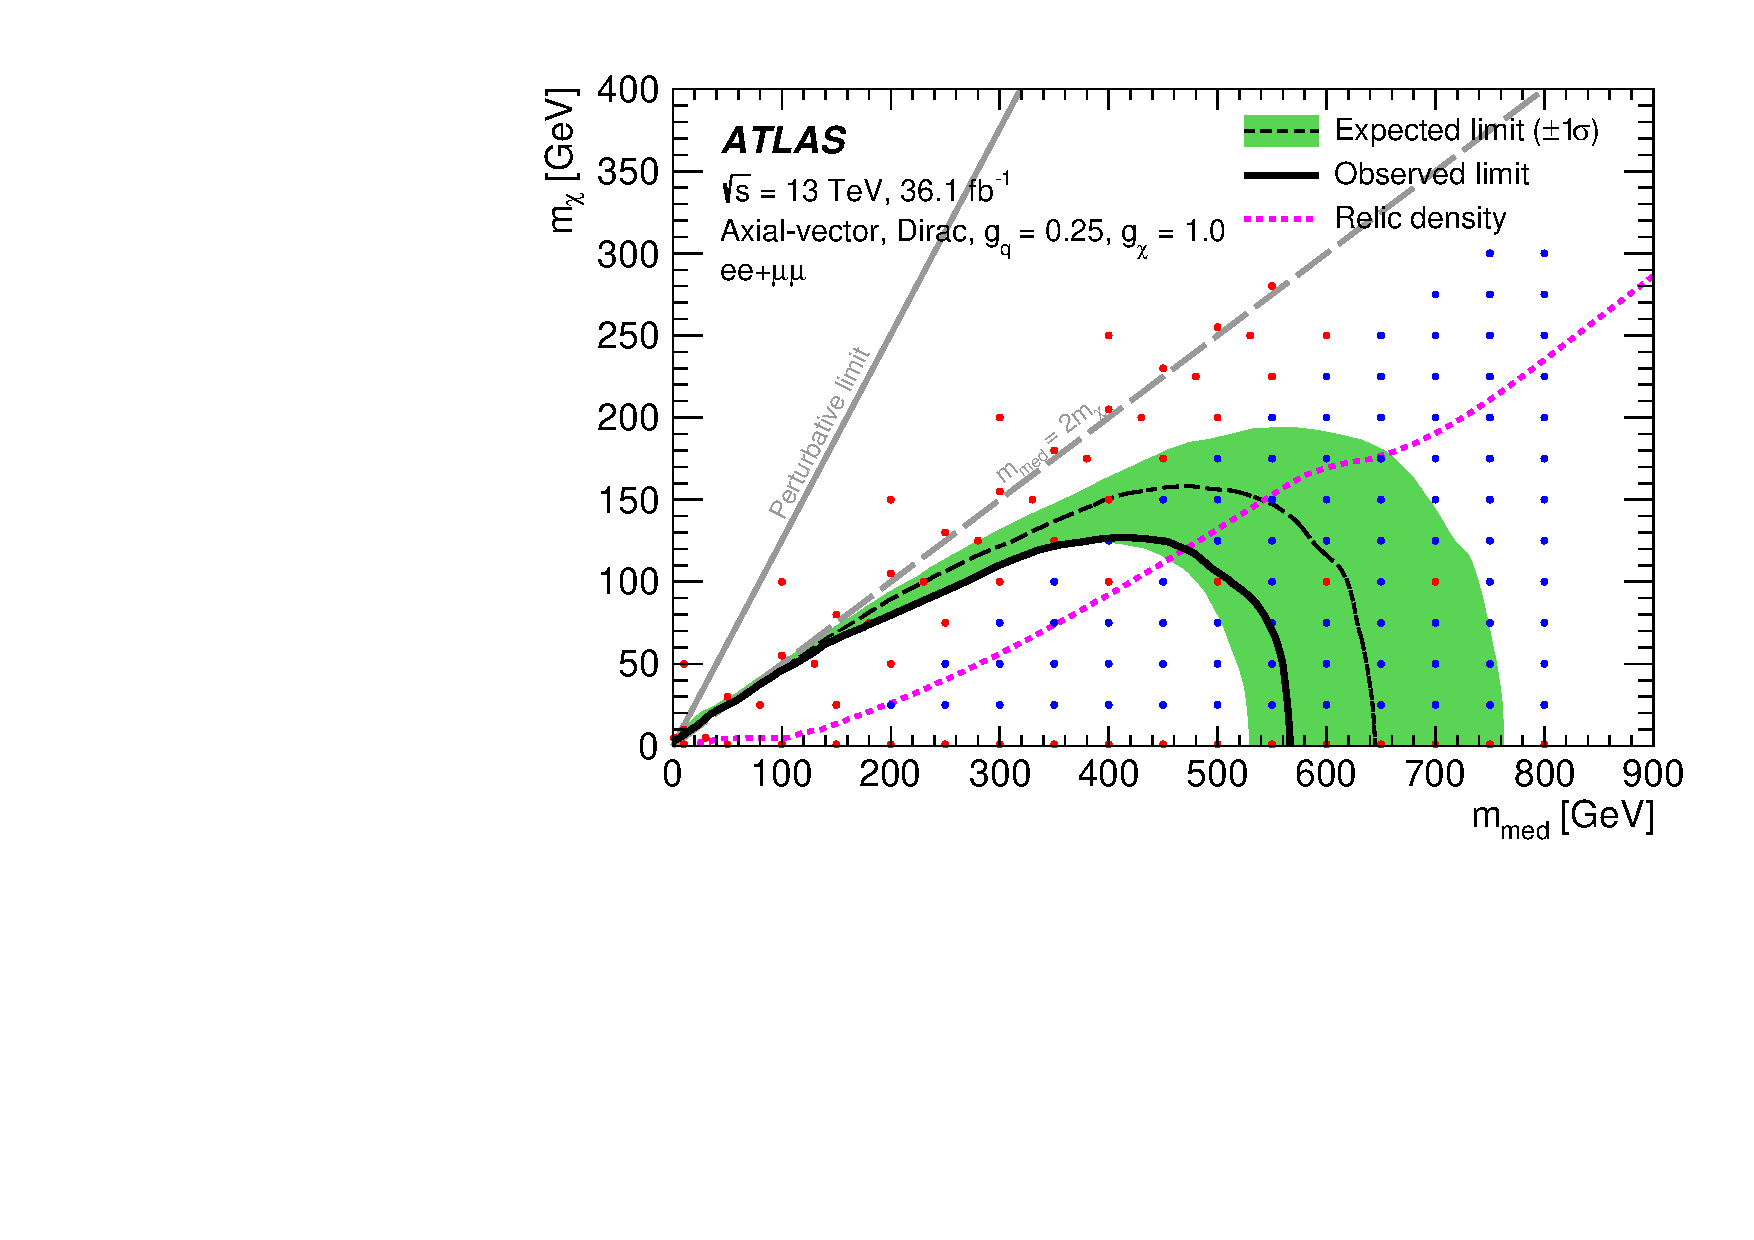
\includegraphics[width=\textwidth]{Figures/limits_dmA.pdf}
        \label{fig:limits_dmA}
    \end{subfigure}
    ~ %add desired spacing between images, e. g. ~, \quad, \qquad, \hfill etc. 
      %(or a blank line to force the subfigure onto a new line)
    \begin{subfigure}[b]{0.48\textwidth}
        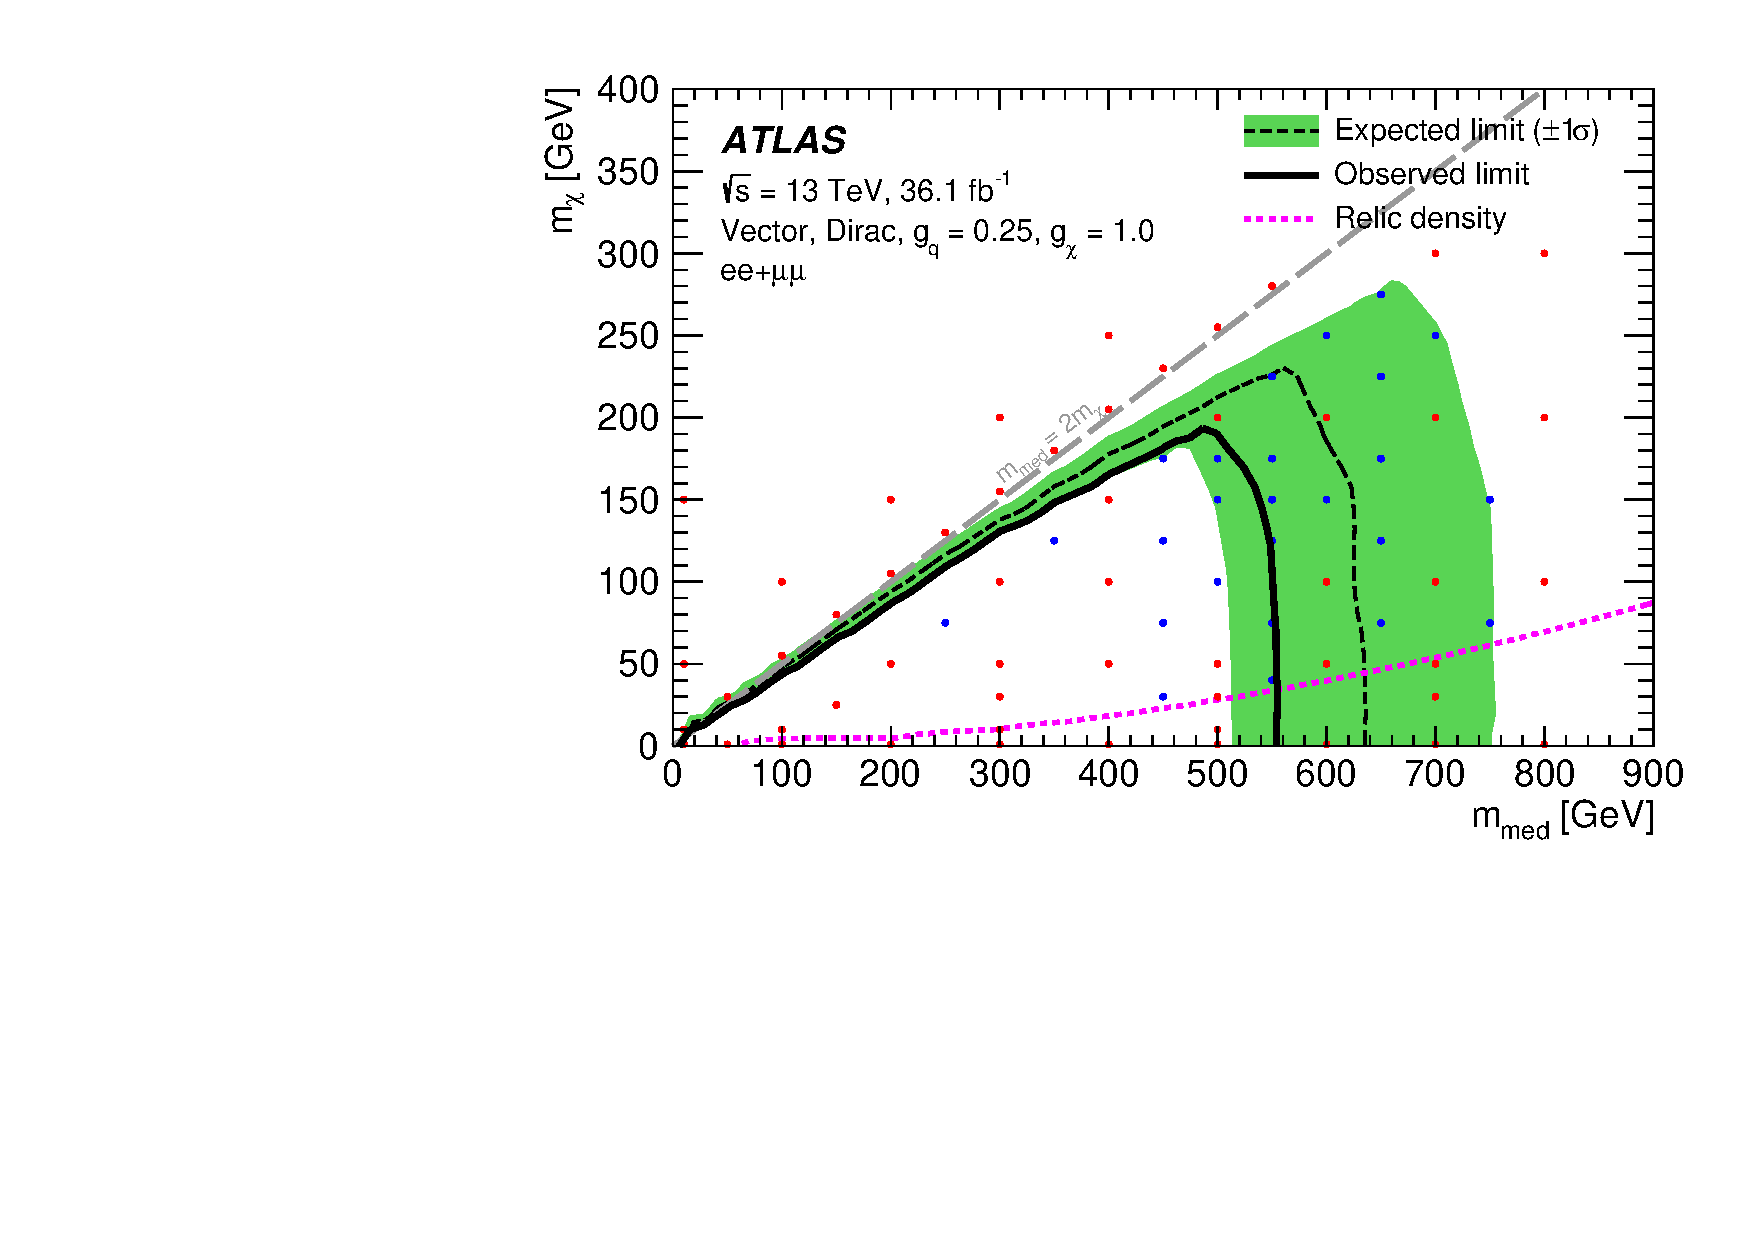
\includegraphics[width=\textwidth]{Figures/limits_dmV.pdf}
        \label{fig:limits_dmV}
    \end{subfigure}
    \caption{Axial-vector (a) and vector (b) exclusion limits on \mchi vs \mmed with 36.1 \ifb.}
\label{fig:limits}
\end{figure}

The 2D mass limits have also been recast into limits on the DM-proton scattering cross section for comparison with DD experiments. The procedure for doing so is given in TODO. Figure \ref{fig:xsec} shows the recast \monoZ limits for the spin-dependent (SD) and spin-independent (SI) scattering cross sections vs \mmed. The cross section is SD if the isotope used in the DD experiment has an unpaired proton or neutron. The limits shown are at the 90\% CL in accordance with the standard used by DD experiments. The coloured lines overlaid are limits set by DD experiments.

\begin{figure}[htb]
    \centering
    \begin{subfigure}[b]{0.48\textwidth}
        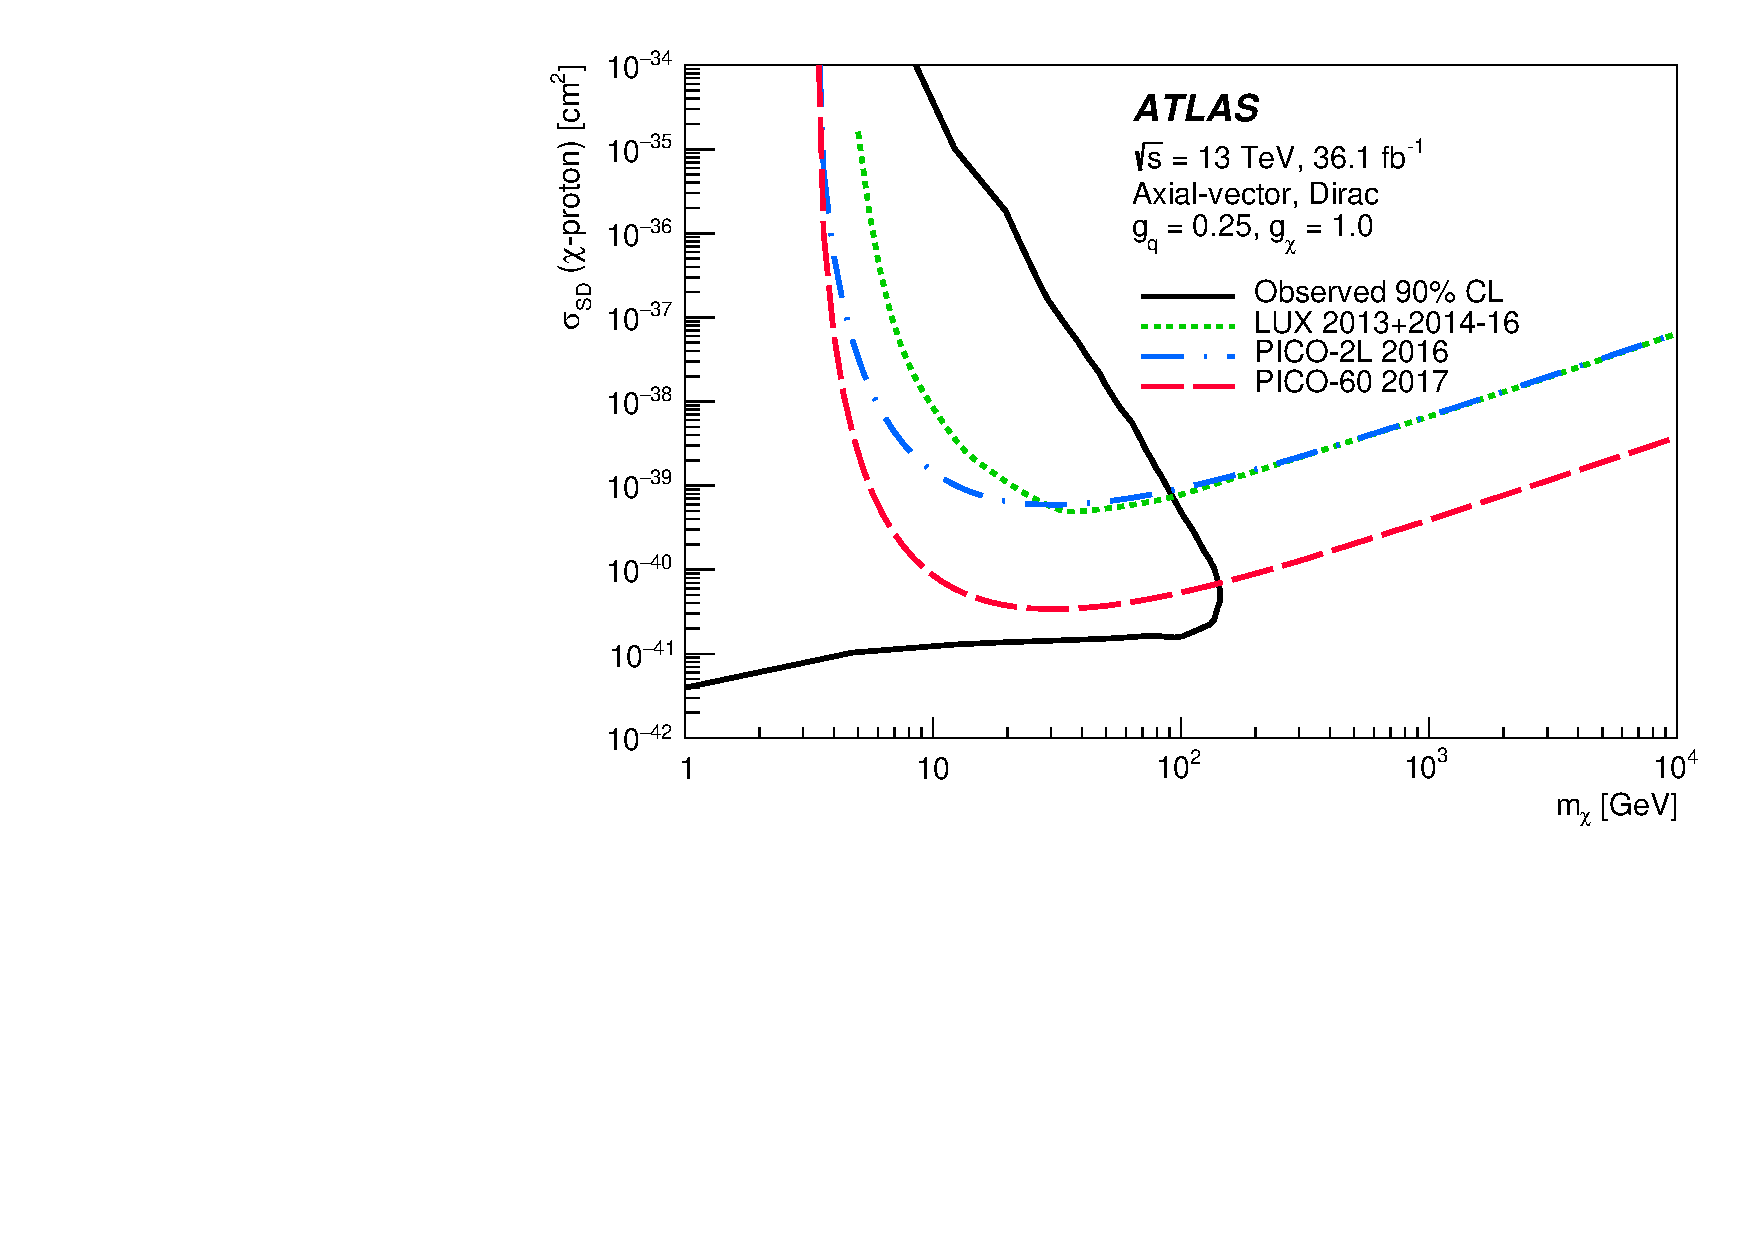
\includegraphics[width=\textwidth]{Figures/xsec_dmA.pdf}
        \label{fig:xsec_dmA}
    \end{subfigure}
    ~ %add desired spacing between images, e. g. ~, \quad, \qquad, \hfill etc. 
      %(or a blank line to force the subfigure onto a new line)
    \begin{subfigure}[b]{0.48\textwidth}
        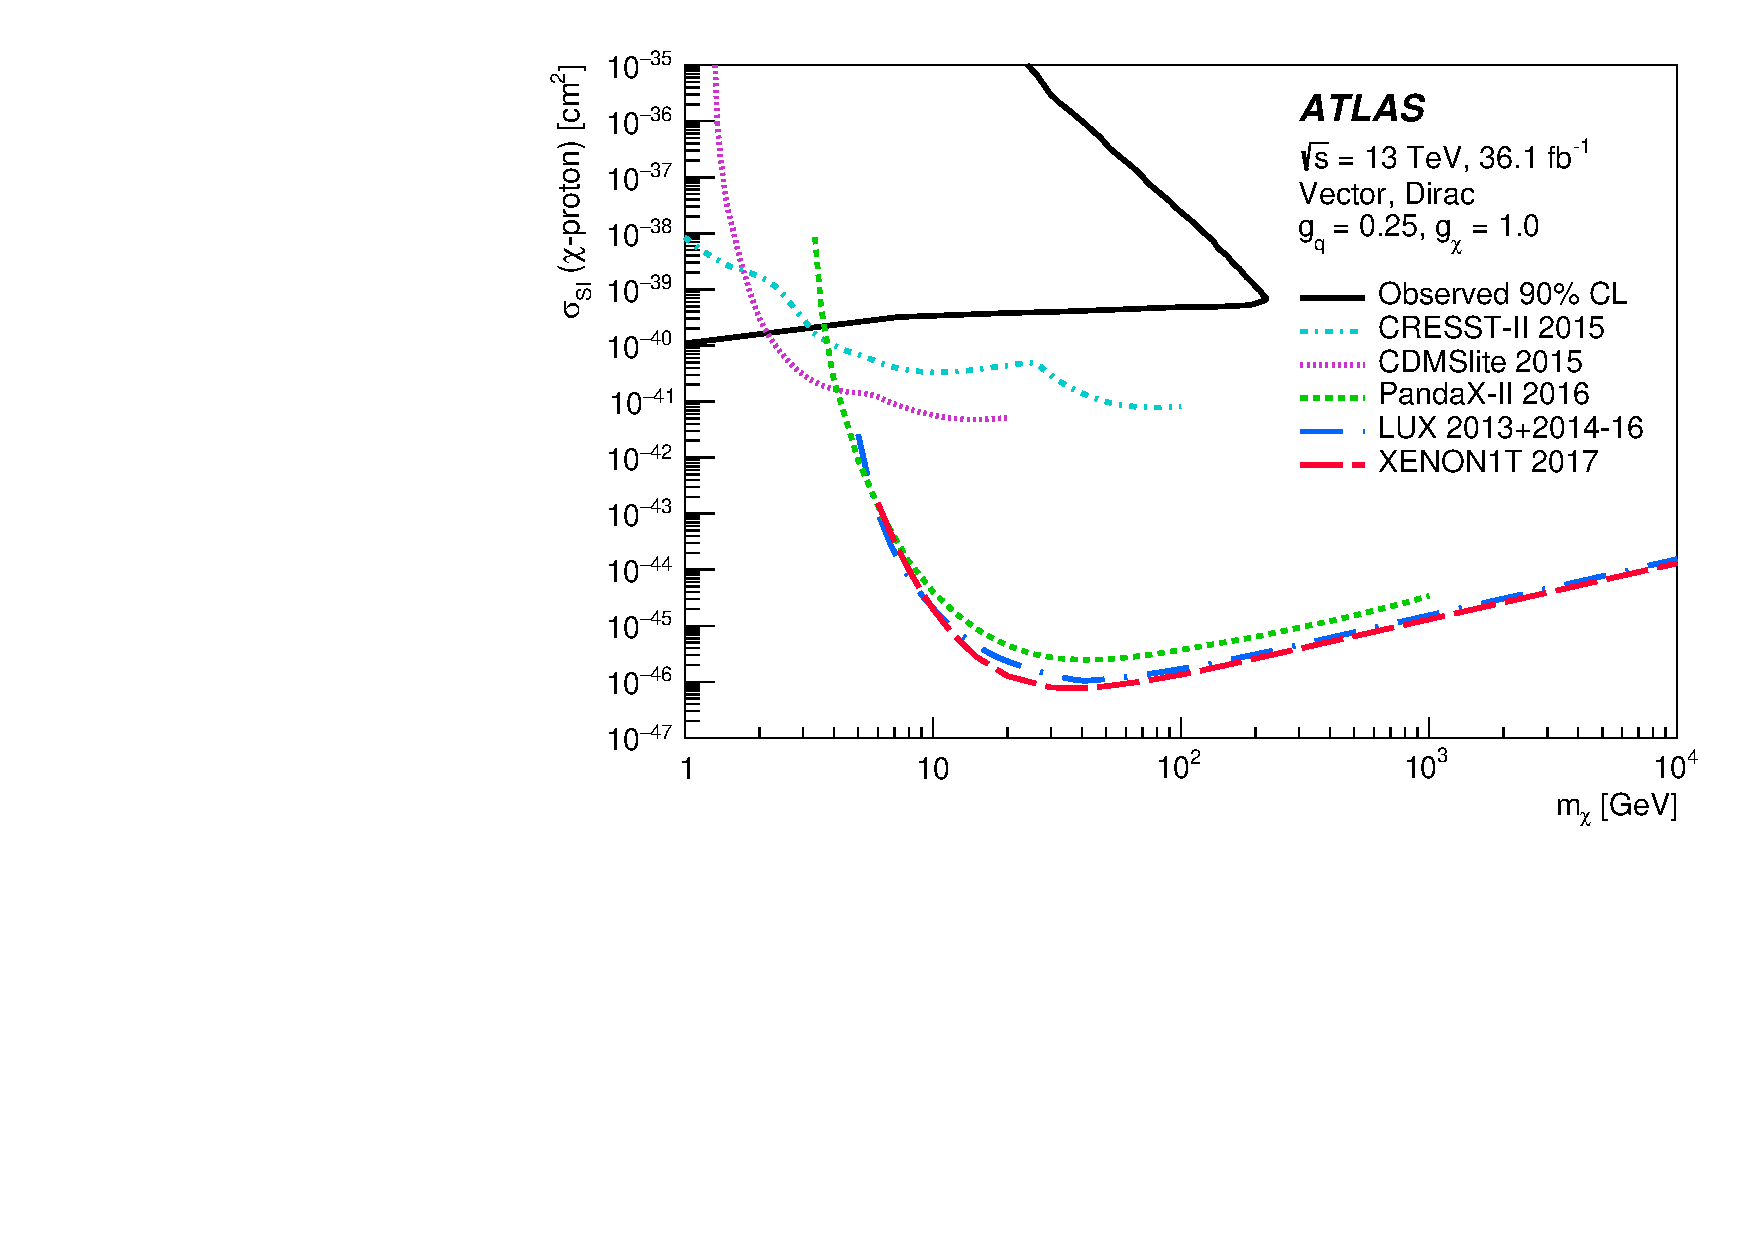
\includegraphics[width=\textwidth]{Figures/xsec_dmV.pdf}
        \label{fig:xsec_dmV}
    \end{subfigure}
    \caption{Axial-vector (a) and vector (b) exclusion limits on the DM-nucleon scattering cross section vs \mmed with 36.1 \ifb.}
\label{fig:xsec}
\end{figure}

Exclusion limits on the 2HDM+PS model have also been set with the 2015+2016 dataset. These are shown in Figure \ref{fig:2hdma}. Limits are set on $m_H$ vs $m_a$ as well as $\tan(\beta)$ vs $m_a$.

\begin{figure}[htb]
    \centering
    \begin{subfigure}[b]{0.48\textwidth}
        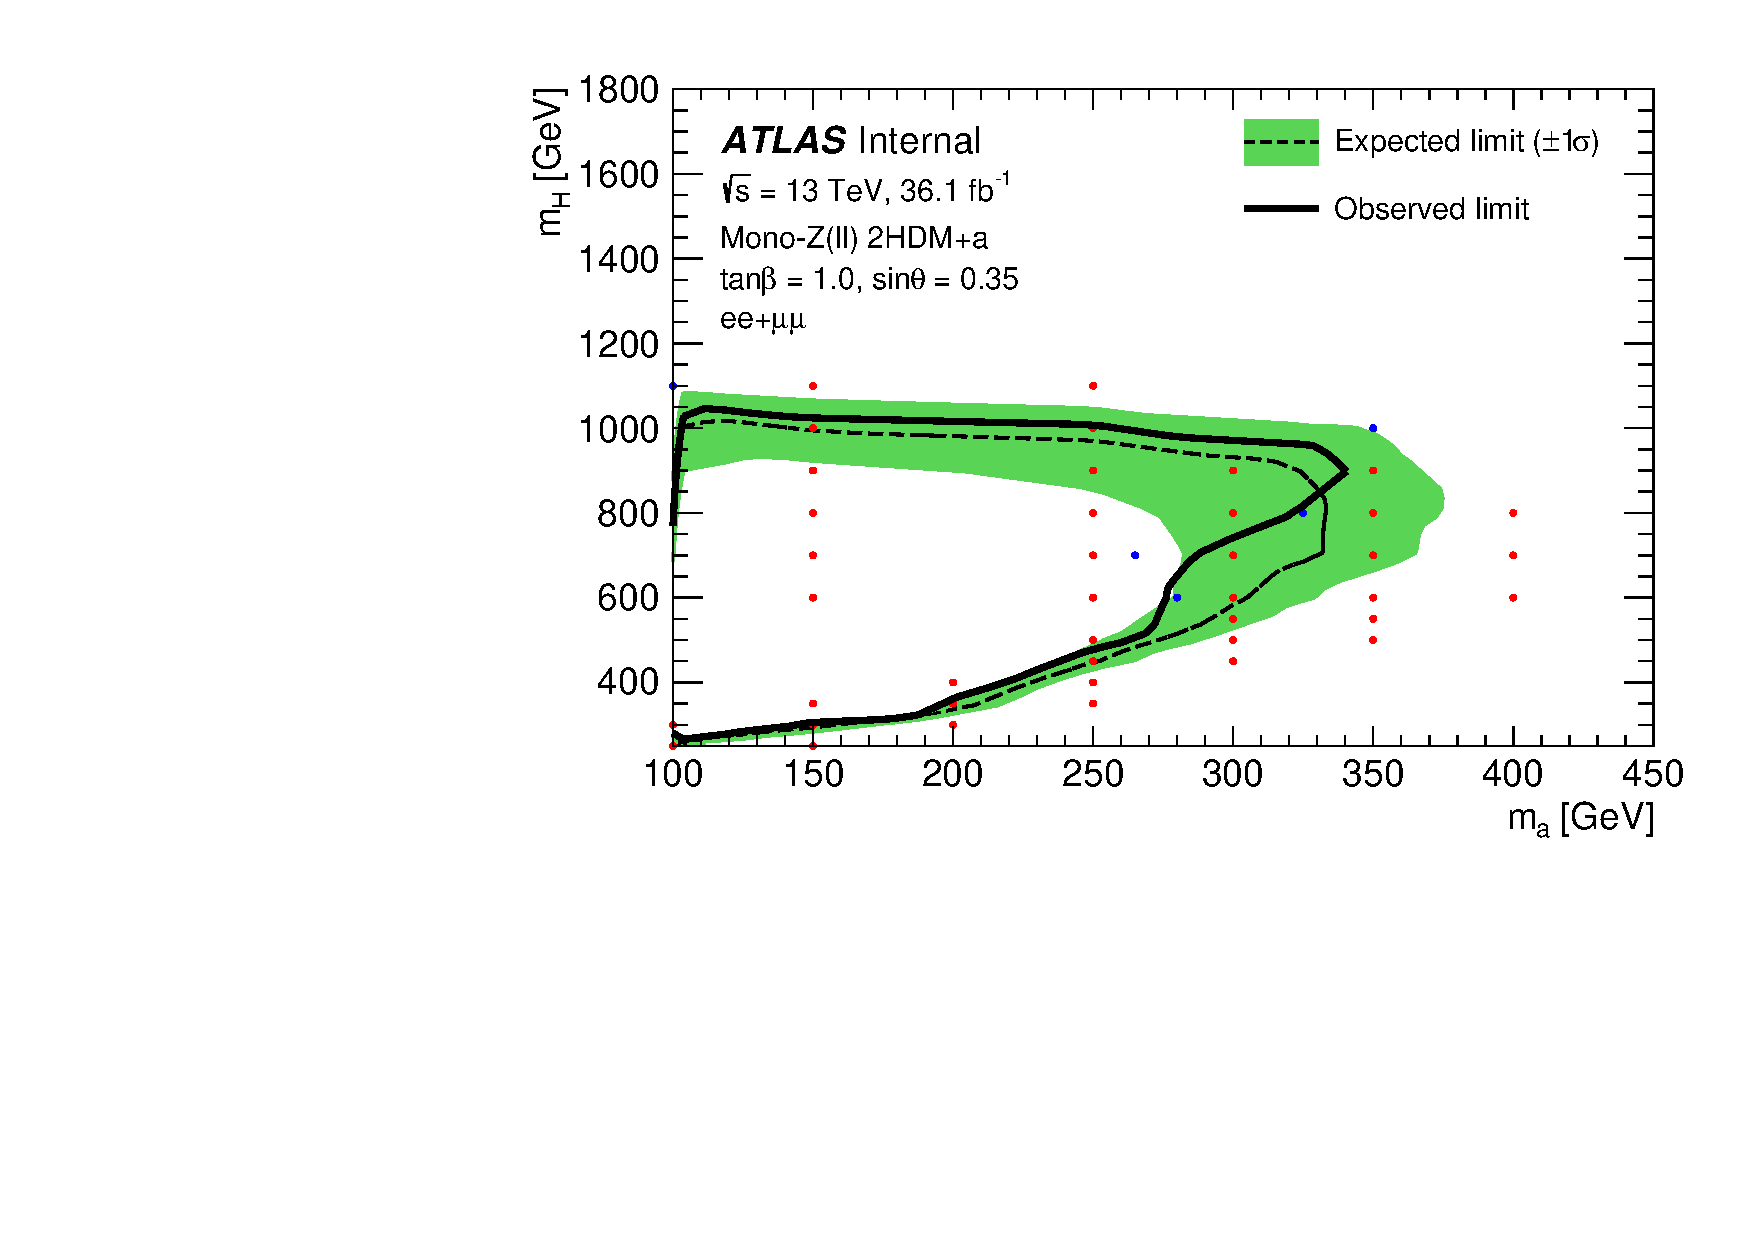
\includegraphics[width=\textwidth]{Figures/limits_2hdma.pdf}
        \label{fig:limits_2hdma}
    \end{subfigure}
    ~ %add desired spacing between images, e. g. ~, \quad, \qquad, \hfill etc. 
      %(or a blank line to force the subfigure onto a new line)
    \begin{subfigure}[b]{0.48\textwidth}
        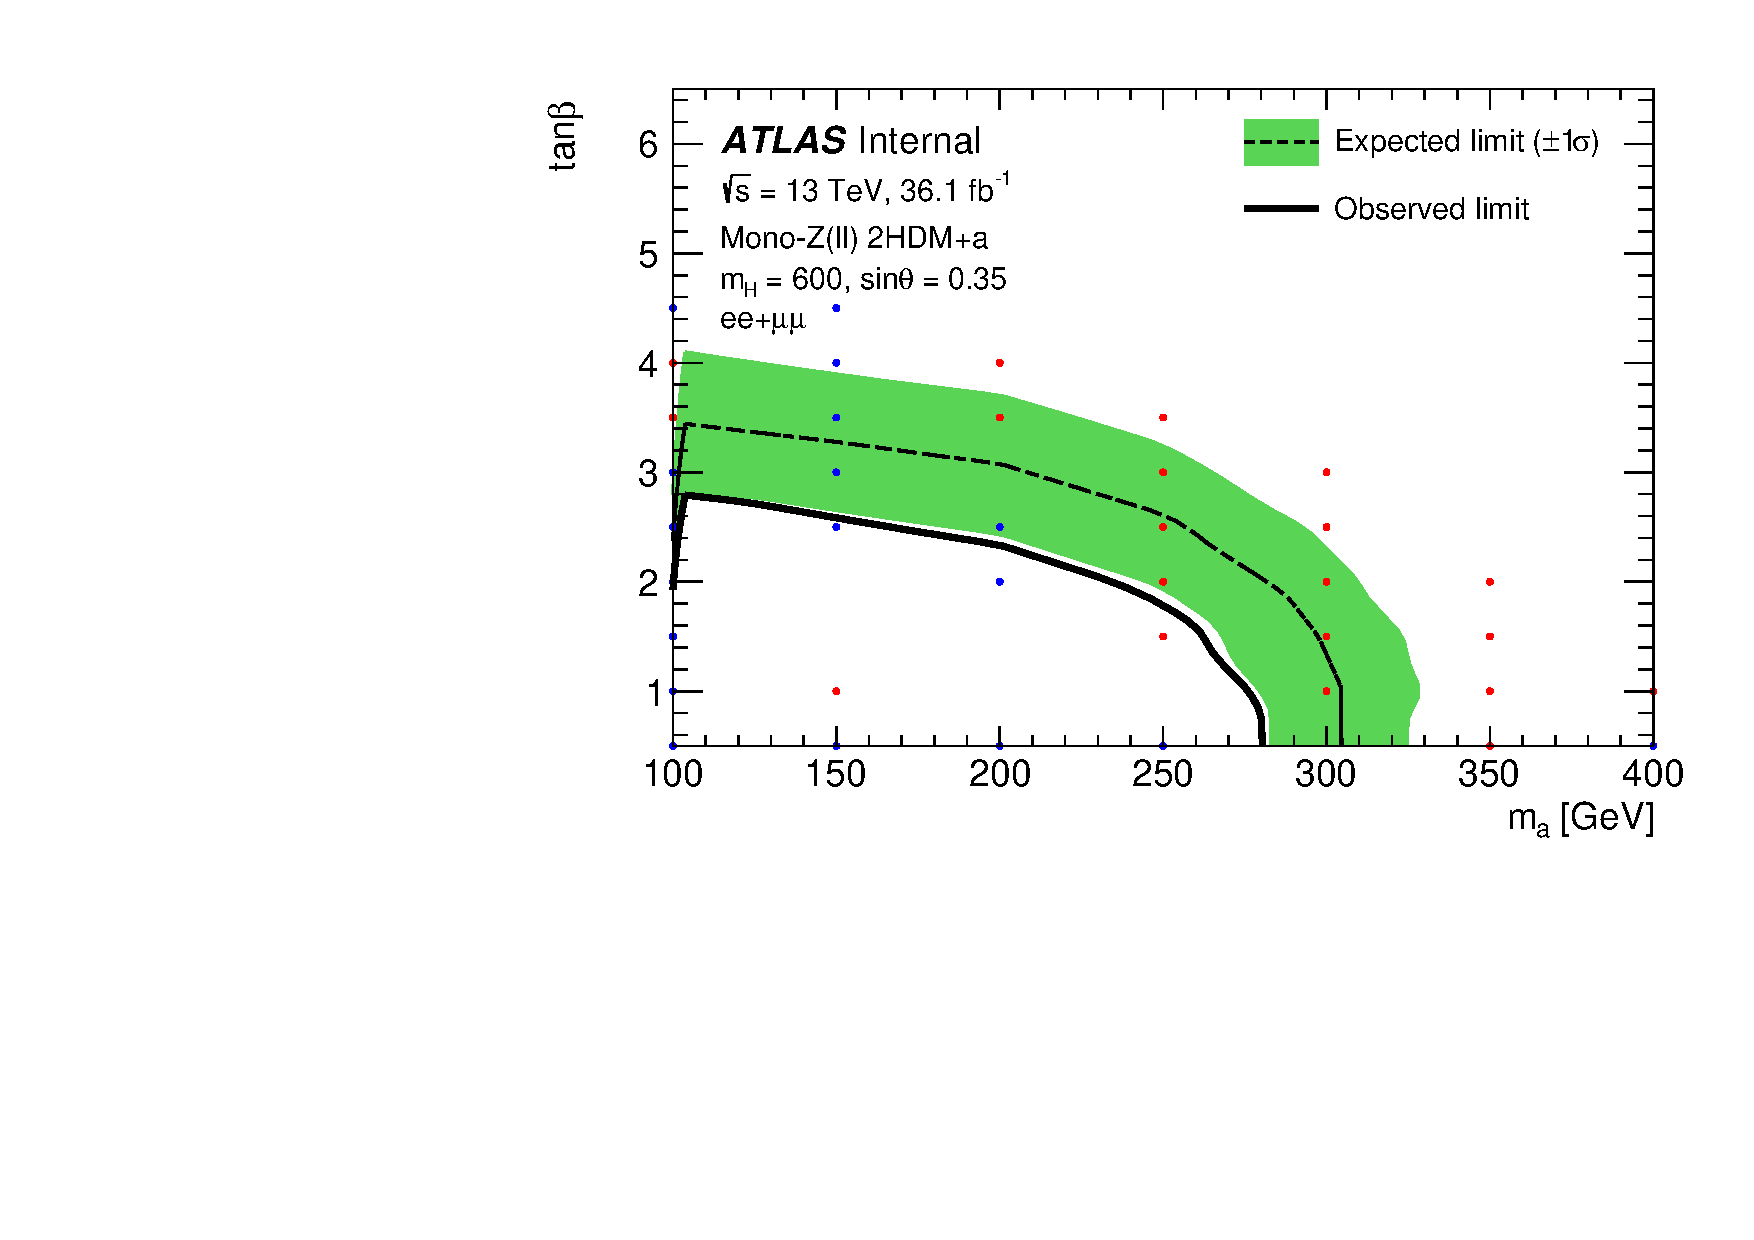
\includegraphics[width=\textwidth]{Figures/limits_2hdma_tan.pdf}
        \label{fig:limits_2hdma_tan}
    \end{subfigure}
    \caption{$m_H$ vs $m_a$ (a) and $\tan(\beta)$ vs $m_a$ (b) exclusion limits with 36.1 \ifb.}
\label{fig:2hdma}
\end{figure}

In the mass limits above, the red points indicate the masses at which there are reconstructed signal samples. The blue points indicate \textit{emulated} points. Mass point emulation is performed to create a finer grid of signal samples without using reconstructed samples. The exclusion contour may look jagged in areas with a coarse grid of signal points. By adding in emulated points, the contour can be made smoother and more physical without going through the tedious process of requesting additional reconstructed MC samples. The method discussed here has been used for the LO simplified models with 36.1 \ifb; emulation for the 2HDM+PS model is more complicated and is not discussed here. 

The validity of emulating signal samples relies on the assumption that the kinematics (i.e. the \etmiss distributions) of the signal does not depend on \mchi in the on-shell region (where $m_\text{med} > 2 m_\chi$). If this is true, then the $E_T^{miss}$ distribution for a reconstructed sample at a given \mmed can be used as the \etmiss distribution for other signal samples with the same \mmed. However, the \etmiss distribution for the emulated sample must be scaled by the ratio of cross sections $\sigma_\text{reco}/\sigma_\text{emul}$. So, as long as the grid of reconstructed points is fine along \mmed, additional points with different \mchi can be emulated just by using the cross sections.

For the axial-vector model, studies on the signal acceptance were been performed and verified that the signal acceptance is flat for a fixed \mmed. For the vector model, an additional complication was that we had a fairly coarse granularity of reconstructed points along \mmed. Because of this, we exploited the similar kinematics between the axial-vector and vector signals and performed emulation from axial-vector $\rightarrow$ vector samples. Emulation for both models has become customary in the \monoZ analysis and will continue to be used moving forward towards the full dataset.


% --------------------------------------------------------------------------------------
\section{Analysis Software}
\label{sec:code}

The MonoZUVic software package is the core of the analysis and has been developed by the UVic group for the past few years. Throughout the evolution of the analysis, contributions have been made towards writing and maintaining the software. The software must be capable of running the entire analysis, including object (electron, muon, jet) calibrations/corrections/selections, removal of overlaps between objects, applying event selections, calculating event weights and kinematic variables, evaluating experimental systematics, and in the end producing trees/histograms for data and MC. Things like calibration recommendations and data formats are in flux quite frequently, and diligent efforts are made to keep the code updated. The software is also cross checked with other groups running the analysis to ensure updated calibrations, squash bugs, etc. The MonoZTruthUVic and MonoZLimitsUVic packages, mentioned briefly above, were written to perform truth-level studies and produce exclusion limits. These packages are also be maintained alongside MonoZUVic. Contributions have also been made to design overhauls in the framework as the analysis has evolved and improved.




	\chapter{Next Steps Towards the Full Run 2 Dataset}

\section{$\gamma$+jets Estimation of the $Z$+jets Background}


\section{$t$-channel Signals}

\subsection{Bell Model}

\subsection{Less Simplified Models}

\section{Analysis Code Framework}
	\startchapter{Conclusions}
\label{chapter:conclusions}

{\color{red}TODO!}
	\appendix
	\startappendix{Appendix}
\label{chapter:appendix}

\section{Event Selections}
\label{sec:evtsel}

Table \ref{tab:sel} summarizes the event selection requirements from the 2015+2016 analysis.

\begin{table}[htbp]
\begin{center}
\begin{tabular}{c|c}
\hline
\hline
Variable  & Requirement  \\
\hline
Lepton pair  &
Exactly one \epem or \mpmm pair with \\
& leading (subleading) \pt > 30 (20) GeV \\
\hline
Third lepton & Veto additional leptons with \pt > 7 GeV \\
\hline
$m_{\ell\ell}$ & 76-106 GeV  \\
\hline
\etmiss & > 90 GeV \\
\hline
$\Delta R_{\ell\ell}$ & < 1.8  \\
\hline
$|\Delta\phi(p_\text{T}^{\ell\ell},$\etmiss)| & > 2.7  \\
\hline
Fractional \pt difference &  < 0.2  \\
\hline
\etmissht & > 0.6 \\
\hline
$b$-jets  & Veto $b$-tagged jets  \\
\hline
\hline
\end{tabular}
\end{center}
\caption{Event selections used for the 2015+2016 result.}
\label{tab:sel}
\end{table}

\noindent Several variables are calculated from the lepton pair. $m_{\ell\ell}$ and $p_\text{T}^{\ell\ell}$ are the invariant mass and the transverse momentum of the pair, and $\Delta R_{\ell\ell}$ is the angular separation between them, where $\Delta R = \sqrt{(\Delta \eta)^2 + (\Delta \phi)^2}$. The fractional \pt difference = $| p_\text{T}^{\ell\ell} - |\vec{E}_\text{T}^\text{miss} + \sum \vec{p}_\text{T}^\text{jets}| | / p_\text{T}^{\ell\ell}$, and $H_\text{T} = p_\text{T}^\text{jets} + p_\text{T}^{\ell_1} + p_\text{T}^{\ell_2}$.

\clearpage

\section{Calibration Studies on Close-By Jets}

The purpose of this work is to validate the jet calibration performance for $R = 0.4$ \akt EM-scale jets in close-by environments. Studies are done on the jet response and resolution for calibrated, close-by jets in \Pythia 8 dijet MC as a function of \DeltaRmin, jet area, and \fCloseby, variables that are used to assess how close-by a jet is. With minimal jet selections and standard $\DeltaR < 0.3$ truth matching, a significant population of low response close-by jets is observed, primarily at low \pt. Several categories of low response close-by jets are investigated. Of the categories investigated, the most important sources of low response are jets with a multi-matched truth jet (one truth jet matched to several jets), and jets with a bad truth matching. Ghost truth association is studied as a robust alternative to \DeltaR truth matching, which can break down in very close-by environments. After removing different sources of low response and switching to ghost truth matching, good agreement is seen in the response for close-by jets with small \DeltaRmin compared to more isolated jets. However some low response jets with small area and/or large \fCloseby remain. Topology and GSC dependence is investigated for these remaining jets, as well as the correlation between \DeltaRmin, area, and \fCloseby.

% The style of bibliography exemplified here is the "plain",
% normally used in science theses. This is shown
% by the entry {plain} below. Substitute the
% appropriate bibliography style. See also the
% PDF file "InformationOnBibliographyStyles" in this
% directory for more choices.

% The Bibliography file is a BibTex file named
% UVicThesis.bib and called below

	\TOCadd{Bibliography}
	\bibliographystyle{bib/bst/atlasBibStyleWithTitle}
	\bibliography{bibliography}
	%\printbibliography

\end{document}
